%===============================================================================
% Autoři: Michal Bidlo, Bohuslav Křena, Jaroslav Dytrych, Petr Veigend a Adam Herout 2018
\chapter{Úvod}

Optimalizace velikosti obrazových dat pomocí komprese je velkým tématem počítačového světa. Dokáže ušetřit přenosovou kapacitu, stejně tak jako umožnit uživateli rychlejší a plynulejší práci. Práce s daty v nekomprimované podobě je výpočetně i paměťově velmi náročná. Jeden snímek videa s vysokým rozlišení (1920x1080 px) dosahuje v nezkomprimované podobě v barevném prostoru RGB s 8b na pixel velikost 6.2 MB. Při běžné snímkovací frekvenci (24 snímků) se jedná o značný objem dat. Navíc lze využít nedokonalostí lidského oka vzhledem k nepřesnostem obrazové komprese na rozdíl např. od textové. Drobná odchylka v barvě řádově desítek bodů při současných rozlišeních (miliony bodů) hraje naprosto minimální roli oproti chybně interpretovanému znaku v textu. Tato skutečnost poskytuje značné možnosti, zároveň je obtížné zvolit přesnou metriku pro porovnávání kvality zdrojových a zpracovaných dat.\\
Dlouhá léta byl - a stále je - standard komprese obrazových dat formát JPEG. Nároky uživatelů - např. průhlednost nebo bezztrátová komprese - které nebyl formát JPEG schopen uspokojit inspirovaly tvůrce k vytvoření jeho nástupce. 
Výsledkem jejich snahy byl JPEG 2000. Formát, jenž v mnohém staví na základech svého předchůdce. Navíc přidává nové možnosti mezi které patří více kvalit v jednom souboru nebo bezeztrátová komprese. Praxe ovšem ukazuje, že ani skoro po dvou dekádách od svého vzniku se nejedná o široce používaný formát. Dokonce jej některé běžné zdroje obsahu - fotoaparáty nebo scannery - nepodporují. Z části se může jednat o nepochopení trhu autory. JPEG 2000 je tak pokročilý, až je pro běžné uživatele příliš obtížné pochopit jeho možnosti. Existující různé práce obsahující doporučení nastavení \cite{profile} \cite{ndk} \cite{bl}, ale zpravidla jsou zmíněny vhodné hodnoty nastavení v nekompletní formě nebo bez bližšího vysvětlení. \\
Hlavním smyslem této bakalářské práce je proto vytvořit ucelenou řadu doporučení pro práci formátem JPEG 2000 nad rozličnými typy obrazových dat. Nejprve je čtenář seznámen se standardem a základním principem funkčnosti. 
Po přečtení této kapitoly by měl mít čtenář jasno proč používat daný formát, kde leží těžiště výhod a kde naopak zvolit jiný technický prostředek. V následující kapitole je popsána metodika měření a vyhodnocování. Následně jsou ilustrovány výběry vstupních obrazových dat. Autorskou část práce tvoří následující dvě kapitoly. První z nich se zabývá návrhem a implementací testovací knihovny. Kapitola je zakončena informacemi o použitých nástrojích, technologiích a postupech, které umožnily postavit základy pro analýzu a vyhodnocení dat. Pro čtenáře zdaleka nejzajímavější bude druhá z nich. Jsou zde vyšetřeny nejdůležitější možnosti obou knihoven při ztrátové i bezeztrátové kompresi. Z výsledku zde získaných je vytvořena ucelená sada doporučení pro kompresi dat formátem JPEG 2000. 

\chapter{JPEG 2000}
\label{teorie}
Jedná o formát \cite{kniha} - definován normou ISO/IEC 15444 - jenž byl navržen \textit{Joint Photographic Experts Group} v roce 2000 jako nástupce formátu JPEG \cite{jpeg}. Norma je rozdělena na více částí, jenž definují jednotlivé nosné myšlenky a přístupy formátu JPEG 2000. Těchto částí je mnoho, avšak pro účely tohoto textu postačí první dvě. První část (\textit{Core coding system}) definuje celý rámec fungování, popisuje hlavní myšlenky a fundamentální principy. Druhá část (\textit{Extensions}) se zabývá rozšířeními mezi které patří markery, nový formát výstupního souboru .jpx, zpracování videa a pokročilé zpracováváním exotických vstupní dat a formátů.

\section{Porovnání s předchůdcem}
JPEG 2000 nabízí mnohé výhody oproti svému předchůdci. Pro uživatele je velice citelnou změnou podpora alfa kanálu (průhlednosti) a kompletní implementace bezeztrátové komprese, kvůli které byla často používán formátu PNG. Uživatel zároveň dostává do rukou mnohem flexibilnější nástroj z hlediska nastavení jednotlivých možností komprese a dekomprese. Pokročilejší kódovací algoritmus zajišťuje lepší kvalitu při zachování stejné velikosti datového toku. S tímto fenoménem jdou ruku v ruce markery, které umožňují dekompresním nástrojům rozbalit pouze zadanou kvalitu, či dokonce region bez nutnost výpočetně náročné dekomprese celého obrazu. I přes značnou podobnost základní funkcionality není zpětně kompatibilní. Zároveň je výpočetně i paměťově náročnější. Nejprve budou osvětleny Jelikož v mnohém staví na své předchůdci je nejprve vhodné si osvětlit základní principy fungování formátu JPEG. 

\begin{figure}[hbt!]
  \hspace*{-0.5cm}
  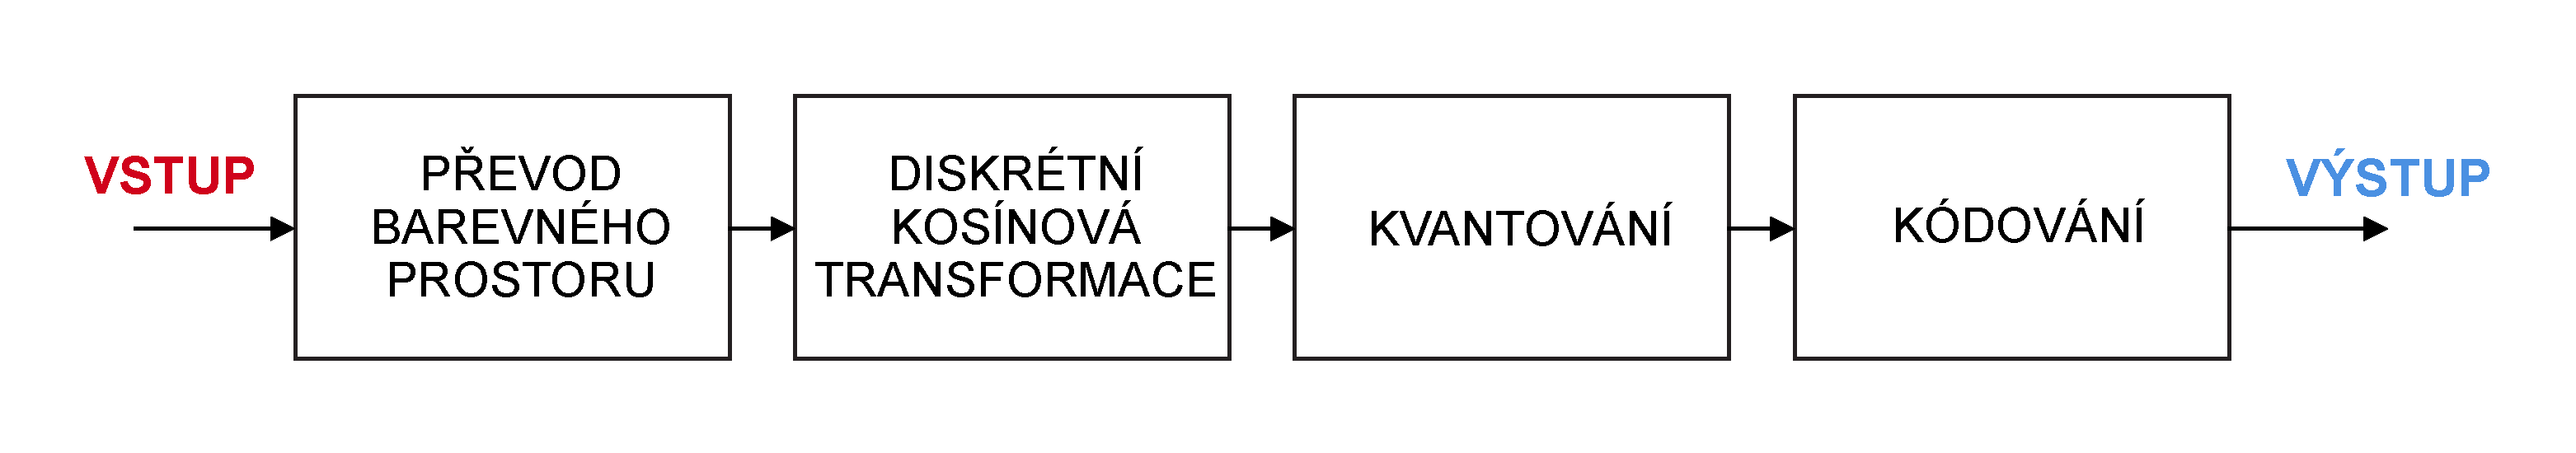
\includegraphics[width=16cm]{obrazky-figures/Artboard.pdf}
  \caption{Zjednodušený řetězec komprese JPEG.}
  \label{retezec}
\end{figure}
 První krok komprese zdrojových dat je transformace barevného prostoru z RGB do YCbCr. Výsledkem jsou tři složky obrazu: jas a barvonosné komponenty (modrá a červená). Barvonosné složky jsou poté podvzorkovány. Následně je obraz v přetransformovaném barevném prostoru rozdělen na bloky velikosti $8x8$ px z důvodu úspory výpočetních zdrojů. Nad touto datovou strukturou je provedena Diskrétní kosínová transformace (DCT). Jedná se o matematický aparát pro vyjádření libovolného signálu signály známými a dobře výpočetně zpracovatelnými. Výsledkem tohoto kroku je matice koeficientů o rozměru $64x64$. Následuje proces kvantování. Jedná o jedinou - pokud je zaručena dostatečná přesnost DCT a použit bezeztrátový převod barevného prostoru - část komprese, která je ztrátová. Jak již bylo zmíněno v úvodu, při tomto kroku využívány vlastnosti lidského oka. Je citlivé na malé změny jasu na velkých plochách, nicméně ne moc dobré v určování konkrétní síly jasu hran (ostré přechody v jasové složce). Tyto přechody jsou reprezentovány jako vysoké frekvence, které lze vhodně omezit či dokonce vynechat. V praxi je tento proces proveden dělením matice koeficientů maticí kvantizační a zaokrouhlením nově vzniklých koeficientu. Kvantizační matice ovlivňuje kvalitu komprese. Posledním krokem je zakódování koeficientů do datového toku. Z matice jsou vybrány metodou zig-zag, následně je tato posloupnost zakódována pomocí \textit{Run-Length} (RLE) kódování, které dobře funguje pro shluky stejných znaků. V tomto případě dlouhé posloupnosti nulových koeficientů vysokých frekvencí. Kód je poté znovu zakódován pomocí Huffmanova kódování a následně složen jako výstupní zkomprimovaný soubor.
Dekomprese je z velké části inverzní proces, pouze je třeba doplnit matice bloků $8x8$, jelikož vysokofrekvenční koeficienty byly při kompresi zahozeny. Předchozí popis jasně demonstruje značnou neflexibilitu formátu. V praxi jediné, co uživatel může ovlivnit je kvantizační matice (tabulka) pro nastavení kvality. 

\begin{figure}[hbt!]
  \hspace*{-0.5cm}
  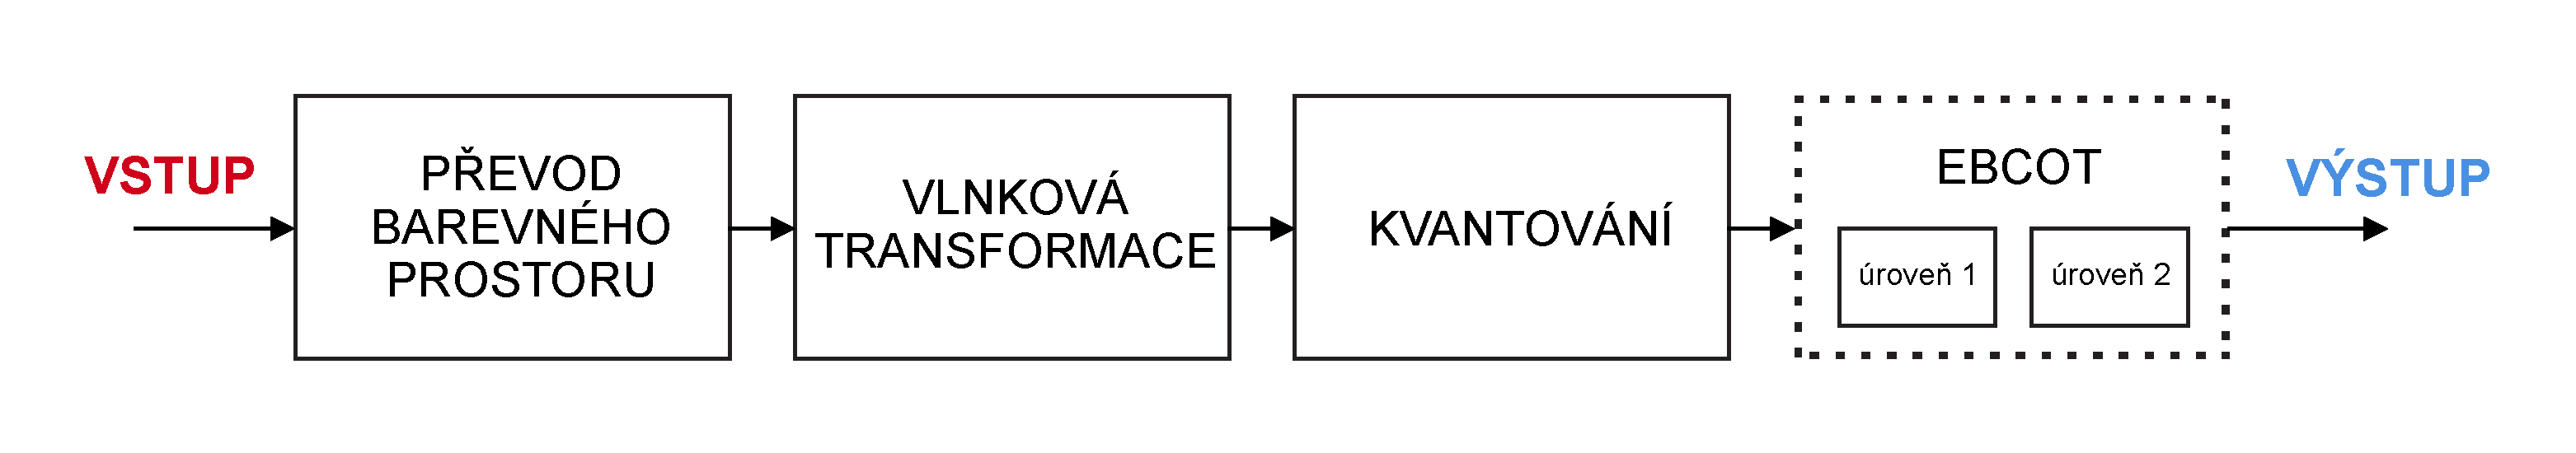
\includegraphics[width=16cm]{obrazky-figures/Artboard2.pdf}
  \caption{Zjednodušený řetězec komprese JPEG 2000.}
  \label{retezec}
\end{figure}

\section{Řetězec zpracování}
JPEG 2000 se snaží v mnoha ohledech tuto neflexibilitu odstranit a nabídnout uživateli větší míru kontrolu nad procesem. Základní stavební bloky komprese jsou podobné jako u předchůdce, jejich přesné fungování je v mnohém odlišné.
\subsection*{Transformace barevného prostoru a podvzorkování}
Ačkoliv většina implementací umožňuje explicitně vynutit vynechání transformace barevného prostoru, pouze málokdy je k tomu dobrý důvod. Hlavním smyslem je odstranit nekonzistence v prostoru RGB. Velmi často dochází ke změnám jednotlivých složek pixelů v nejbližším okolí. Ačkoliv se může jednat o změny velmi malé, při nevhodně zvolené velikosti zpracovávaného bloku dochází ke vzniku blokových artefaktů.\\
Standardně používaným barevným prostorem je YCbCr, kde Y značí luminanci (jas), a Cb/Cr chrominanci (barvonosné složky - červená, respektive modrá). Všechny důležité informace o obrazu jsou reprezentovány ve složce Y, což reflektuje citlivostí profil lidského oka \cite{oko}, odstraňuje chyby barevné nekonzistence a zjednodušuje následné zpracování. Nakonec je důležité zmínit, že se nejedná o absolutní barevný prostor. Výsledný datový tok může být např. závislý na barevném profilu. Barvonosné složky podvzorkovat (např. 4:2:2, kdy dojde ke dvojnásobnému podvzorkování u barvonosných složek, ale luminance zůstane nedotčena).\\
Transformace lze provést ve dvou módech. Buď ztrátově (\textit{Irreversible Component Transform} - ICT) v artitmetice s plovoucí desetinnou čárkou.
\begin{gather}
 \begin{pmatrix} Y \\ C_b \\ C_r \end{pmatrix}
 =
 \begin{pmatrix} 0.299 & 0.587 & 0.114 \\ -0.16875 & - 0.33126 & 0.5 \\ 0.85 & - 0.41869 & -0.08131 \end{pmatrix}
.
 \begin{pmatrix} R \\ G \\ B \end{pmatrix}
\end{gather}

\noindent A nebo bezeztrátově (\textit{Reversible Component Transform} - RCT) v celých číslech.
\begin{gather}
 \begin{pmatrix} Y \\ C_b \\ C_r \end{pmatrix}
 =
 \begin{pmatrix} \floor*{\frac{R + 2G + B}{4}} \\ \floor*{B - G} \\ \floor*{R - G} \end{pmatrix}
\end{gather}

\subsection*{Rozdělení obrazu}
Zde probíhá první velký odklon od JPEG. U něj jsou normou definované bloky $8x8$ px, které jsou samostatně zpracovávány. Jeho nástupce nabízí mnohem jemnější dělení a kontrolu nad procesem. V průběhu celé práce je možno se setkat s trojicí pojmů označují dělení obrazu. Jsou to dlaždice (\textit{tiles}), precincty (\textit{precincts}) a kódové bloky (\textit{code-blocks}). Kromě dělby obrazu v této úrovni zpracování existují ještě tzv. regiony zájmu, které určitou část kódují prioritně. Tento proces probíhá po provedení vlnkové transformace.

\begin{figure}[hbt!]
  \hspace*{-0.5cm}
  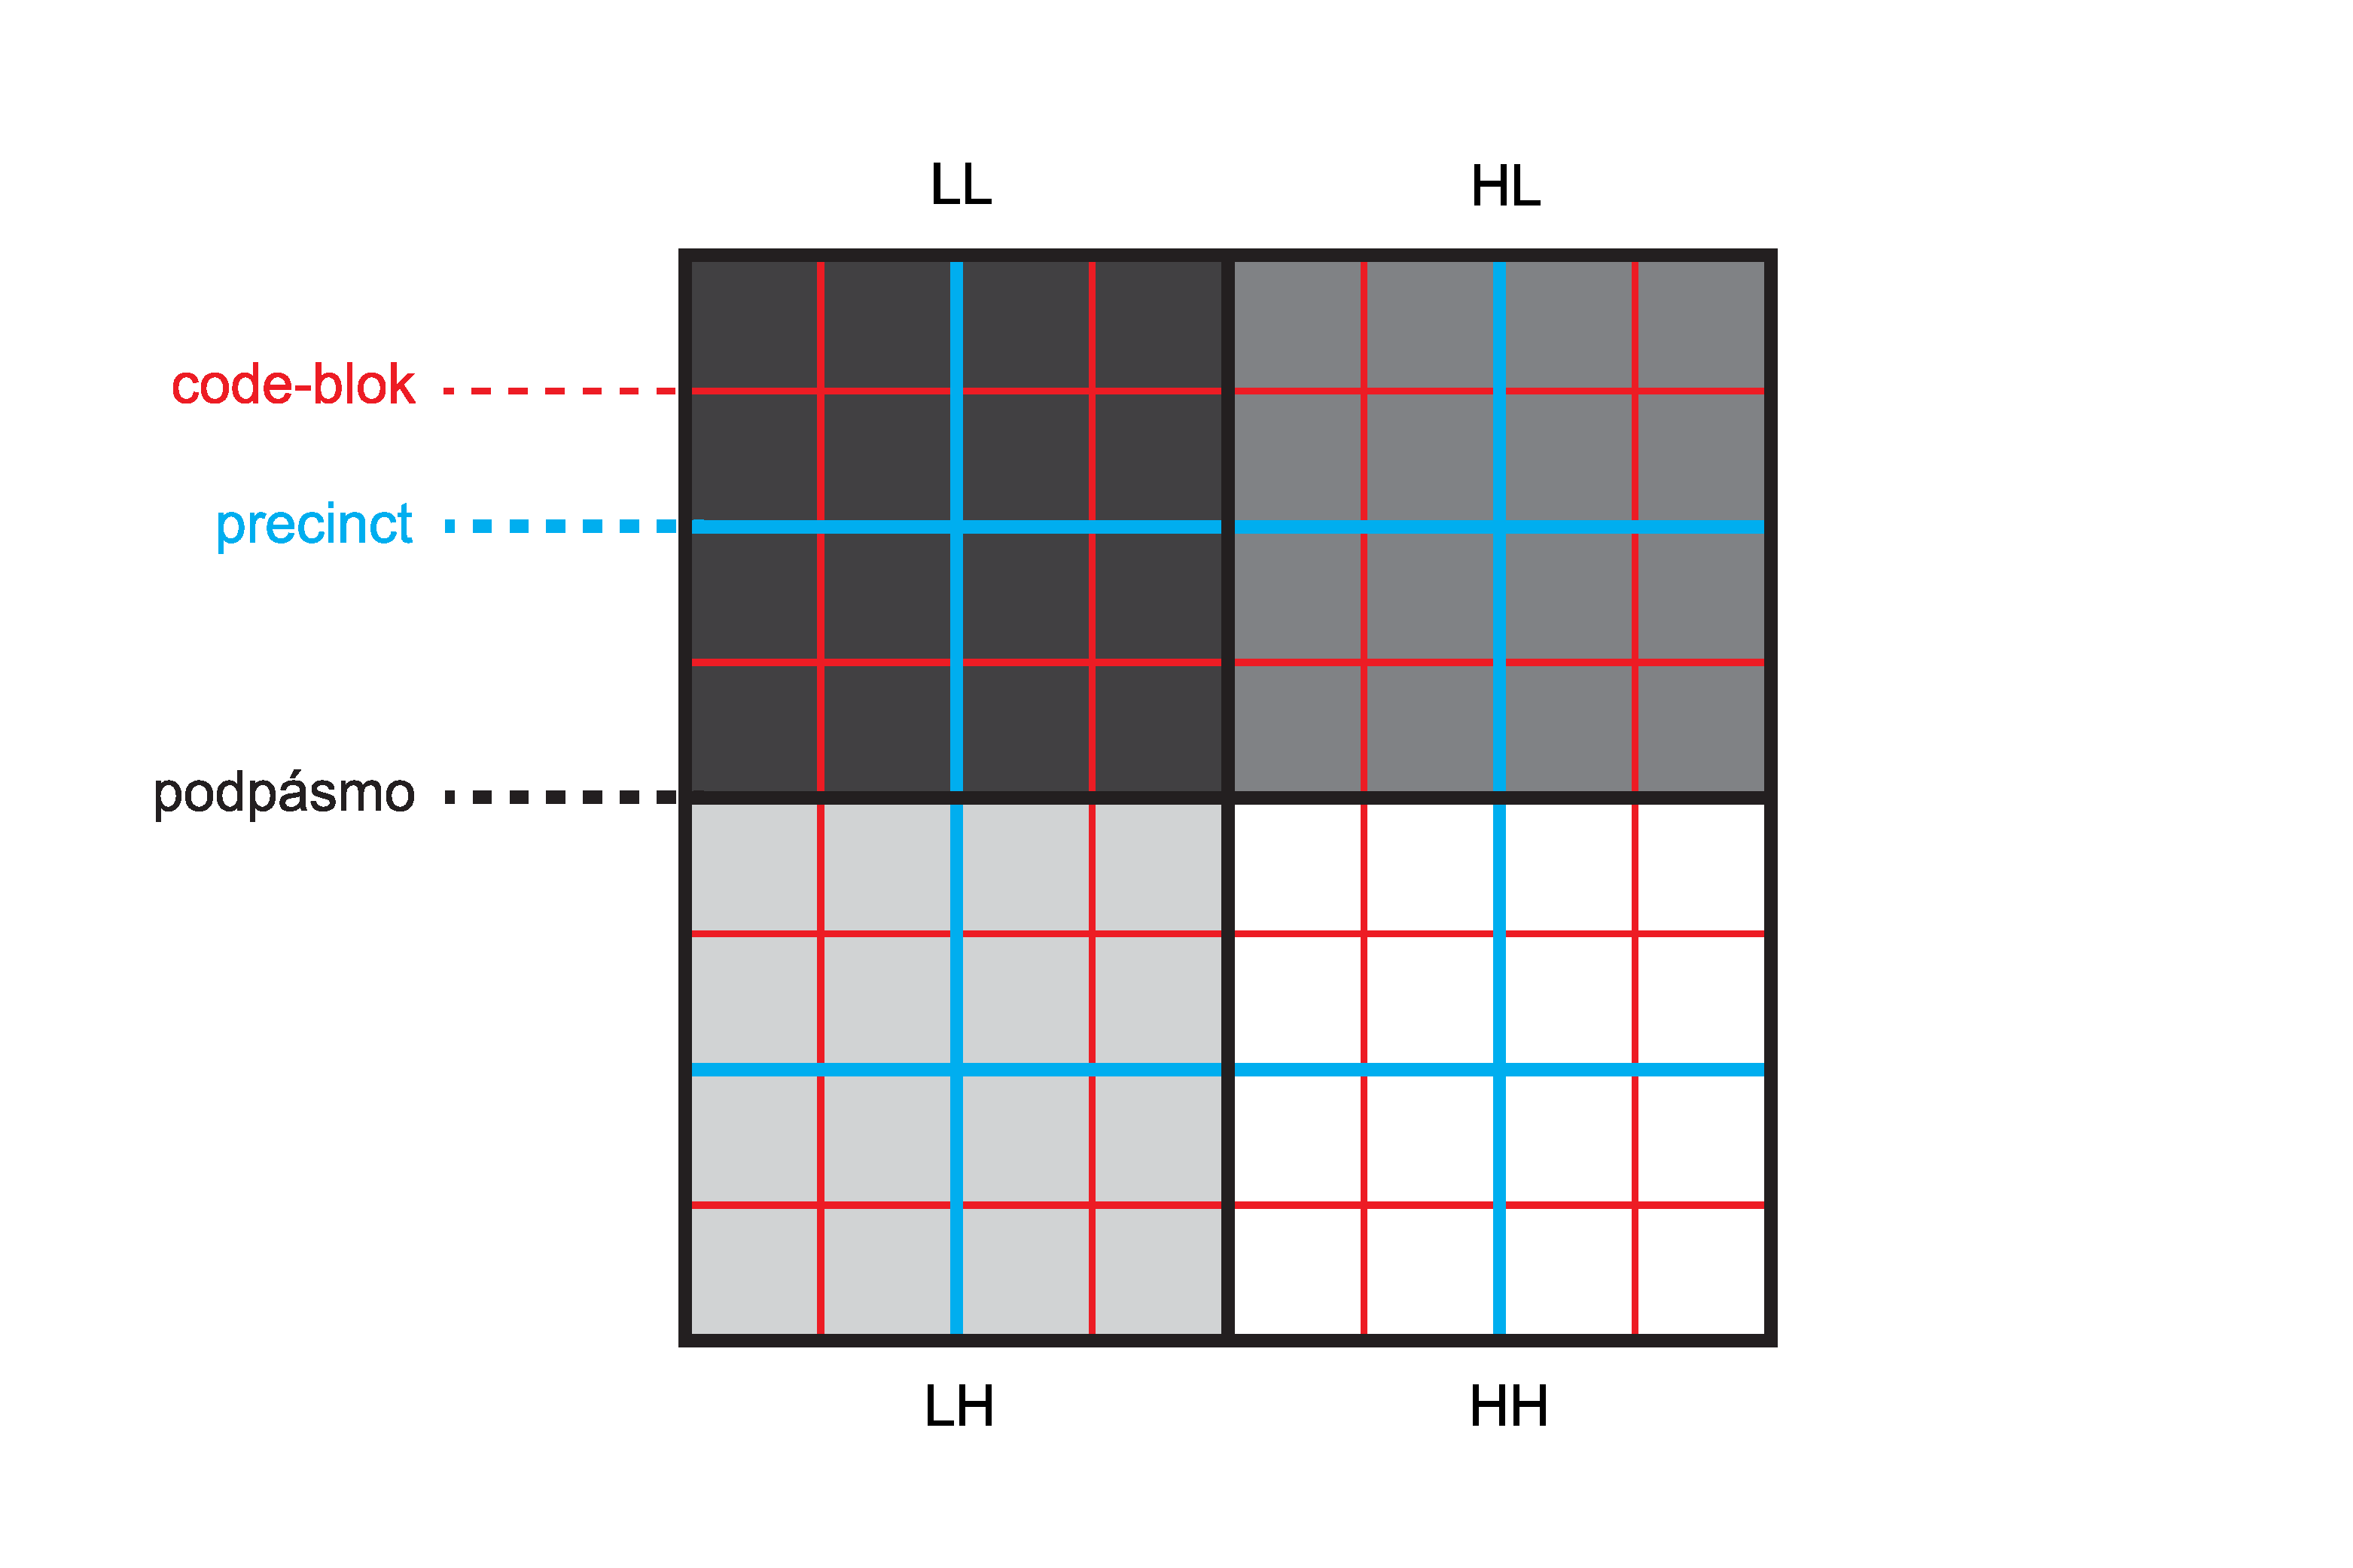
\includegraphics[width=16cm]{obrazky-figures/tiles.pdf}
  \caption{Nástroje pro dělení obrazu.}
  \label{retezec}
\end{figure}

\noindent Nejprve si nutno vysvětlit nastavené rozměry. Dlaždice z originálního obrazu vyřízne čtvercový blok o velikosti 512x512 px. Ačkoliv jsou v tomto případě voleny přesně čtvercové rozměry dlaždice, je možno zvolit vzájemně nezávislé rozměry s libovolným poměrem stran z splnění podmínky nezápornosti obou rozměrů. Tato vlastnost umožňuje efektivně pokrýt dlaždicemi obrazové data atypických rozměrů. Standard také definuje možnosti posunu dlaždic a obrazu vůči výchozí bodu (levý horní roh). Dělení obrazu na dlaždice lze vypnout. Poté obraz brán jako jedna dlaždice. Obraz je v tomto případě dekomponován pouze jednou. Výsledkem jsou čtyři podpásma o velikosti 256x256 px. Precinct v tomto případě volen o velikosti 128x128 px. Rozměr precinctu je přesně definován jako násobky dvou a může se lišit pro každou dlaždici. Rozměry proto mohou být ušity na míru konkrétní části obrazu rozděleného dlaždicemi. Tento způsob dělení nemá přímý vliv na kvalitu, ale má vliv na velikost datového toku, jelikož každý precinct slouží jako základ pro pakety výsledného datového toku. Každý paket disponuje určitou režií - hlavně při použitých markerech na označení konce a začátku - je nutno velikost vhodně zvolit. Poslední dělící komponentou je blok code-blok o velikosti 64x64 px. Code-bloky slouží jako vstupy kóderu.


\subsection*{Vlnková transformace}
Srdcem komprese je Diskrétní vlnková transformace (DWT) \cite{vlnkova}. Opět se jedná o tvorbu koeficientů na základě vstupních dat \cite{intro}. Hlavní rozdíl oproti \textit{Discrete Fourier Transform} (DFT), potažmo DCT, je použití speciálního signálu (tzv. \textit{wavelet} - vlnka). Ta umožňuje mnohem lépe popsat určitý jev v signálu. Harmonické průběhy mají problém s reprezentací náhlých změn průběhu signálu (hrany v obraze), jelikož nemají jasně vymezený čas (oscilují od $-\infty$ do $\infty$). Naopak vlnka u DWT má jasně vymezený čas a nulovou střední hodnotu.\\
V případě JPEG 2000 je užita vlnka \textit{Cohen–Daubechies–Feauveau} (CDF) ve dvou variantách. Ztrátovou kompresi zajištuje CDF 9/7 operující s plovoucí aritmetice vylučující úplnou zpětnou reprezentaci z důvodu zaokrouhlovacích chyb v případě dekomprese a bezeztrátovou CDF 5/3 pracující na celými čísly. Některé implementace umožňují změnit volbu vlnky nezávisle na typu komprese; tato možnost bude experimentálně vyšetřena. 

\begin{figure}[hbt!]
  \centering
  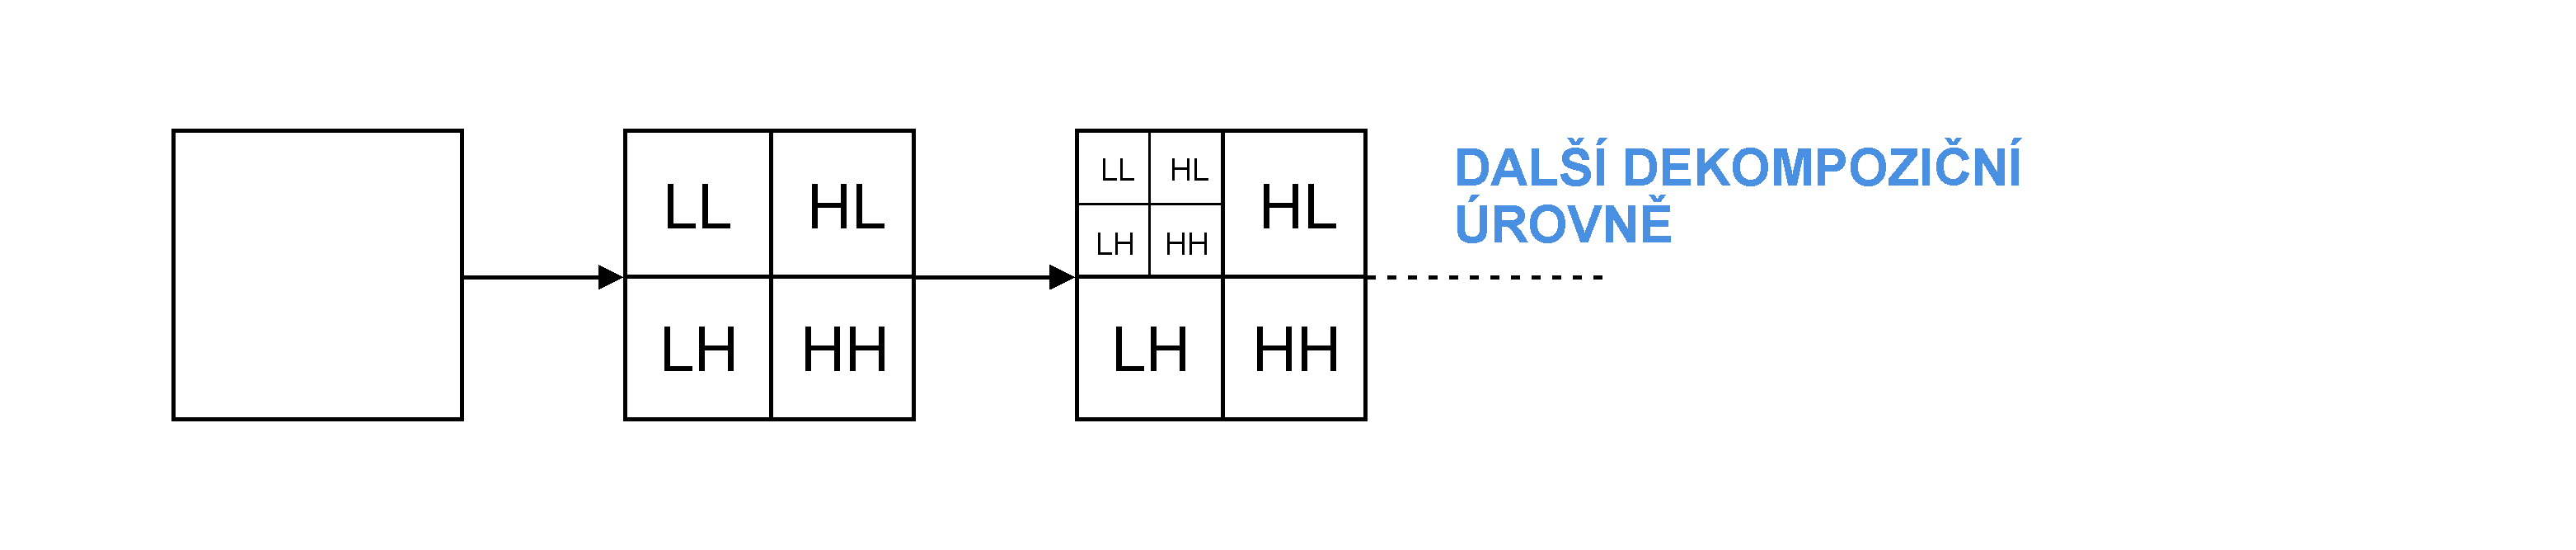
\includegraphics[width=16cm]{obrazky-figures/Artboard4.pdf}
  \caption{Naznačení vícenásobného rozkladu DIT.}
  \label{retezec}
\end{figure}

\noindent Obraz je transformací rozložen na čtyři podpásma, která jsou dále zpracovávána. S každou další úrovní rozkladu je dekomponována nízkofrekvenční složka LL z důvodu citlivost lidského oka na nízké frekvence. Počet úrovní je jeden z nejdůležitějších parametrů ovlivňující kompresní výkon jelikož je zapotřebí najít vhodný počet úrovní, kdy počet podpásem dostatečného počtu pro kvalitní reprezentaci obrazu, avšak ne příliš velký, tak aby způsoboval značné zvýšení výpočetních nároků a zhoršení kompresního výkonu. 


\subsection*{Kvantování}
Kvantování funguje podobně jako u JPEG \cite{qua}. Odstraní nebo omezí složky málo důležité a nepotřebné (zpravidla vysoké frekvence). Na rozdíl od JPEG není použito implicitně vždy, ale pouze při výběru ztrátové komprese. Běžně se používá skalární kvantizace, které funguje na principu odseknutí méně významných bitů koeficientů od určité bitové pozice. 

\subsection*{Kódování}
Tvoří poslední díl skládačky. Slouží k zakódování koeficientů DWT do příslušných datových struktur. Prace s code-bloky, které jsou kódovány nezávisle. Implementačně i principiálně se jedná o mnoho složitější funkční blok než u JPEG. Proto je rozdělen na dvě části.

\subsection*{EBCOT}
\textit{Embedded Block Coding with Optimised Truncation} (EBCOT) \cite{ebcot} popisuje pokročilý algoritmus na správu bitů v toku. 
Obecný princip je následující:
\begin{itemize}
  \item{Rozdělení code-bloků do $n$ bitových rovin, které jsou seřazeny od nejvýše významného po nejméně významný bit.}
  \item{Každá rovina je zakódována třemi průchody, kde každý bit může být vybrán jenom jednou. Pokud je rovina složena pouze z nulových koeficientů je přeskočena, ale je započtena do celkového počtu rovin. Pro každý bit v Code-bloku je vytvořena dvojice proměnných. Binární stav významnosti, nastaven při prvním výskytu hodnoty v koeficientu a vektor stavů významnosti nejbližšího okolí; zde osmiokolí. Kódování probíhá v těchto úrovních:}
  \begin{itemize}
    \item \textit{Significance Propagation Pass} - Bit je zakódován, pokud je nevýznamný, ale alespoň jeden z jeho sousedů významný je.
    \item \textit{Magnitude Refinement Pass} - Jsou zakódovány bity, které již významné byly, stejně tak jak ty označené v předchozím průchodu.
    \item \textit{Clean-up Pass} - Bity, které nebyly zakódovány žádnou z předchozích fází. Tato fáze je zároveň první při začátku průchodů novým code-blokem.
  \end{itemize}
  \item Dvojice informací o významnosti - zde nazýváno symbol pro ukazatel významnosti a kontext pro informace o okolí z předchozího bodu - je zaslána do aritmetického kodéru.
\end{itemize}
Algoritmus zároveň definuje průchod code-bloků. Každý je rozdělen na vodorovné pruhy o výšce $4$ b a svojí původní šířce. Pruhy jsou zpracovávany zhora dolů. Pohyb v pruhu bitů je svislý, zleva doprava. Každý sloupec v pruhu je zpracováván svisle zhora dolů. Aritmetický kodér (dále MQ kodér), který je do značné míry zodpovědný za výsledný datový tok, umožnuje velkou míru nastavení. Z důvodu komplexních algoritmů existují formátem definované předvolby \cite{kniha}:

\begin{table}[ht!]
  \centering
    \setlength{\tabcolsep}{3pt} % Default value: 6pt
    \renewcommand{\arraystretch}{1.15} % Default value: 1

    \begin{tabular}{|p{3cm}|p{11.5cm}|}
      \hline
      \textbf{Typ} & \textbf{Vlastnost} \\ 
      \hline

      BYPASS & Používá pouze aproximace průchodů, může být značně rychlejší za cenu nepatrně horší komprese.\\ 
      CASUAL & Rozdělení zpracované části bitové roviny do pruhu o velikost 4 a zmenšení vlivu budoucích pruhu na současné kódování.\\
      RESET & Vektor významnosti okolí je spočten pouze jednou.  \\ 
      RESTART & MQ kodér je při každém kódovacím průběhu vyčištěn. \\ 
      ERTERM & Zajišťuje přesně definované chování symbolů a kontextu. \\ 
      SEGMARK & Na konec každé bitové roviny je přidána čtyřbitová kombinace. \\
      \hline
    \end{tabular}
    \caption{Možnosti nastavení MQ kodéru.} 
\end{table}


\subsection*{Generování výsledného toku}
MQ kodér tvoří na svém výstupu posloupnost, která se skládá zpět na precincty (nadmnožina code-bloků) formující pakety po přidání hlavičky. Pakety všech podpásem jsou zkomponovány do vrstev. Pořadí paketů ve vrstvě není definováno. Obsah vrstev lze ovlivnit např. pomocí regionů zájmu. Velká výhoda formátu je možnost dynamicky dekódovat obraz po vrstvách - velmi vhodné např. pro pomalé přenosy dat, kdy je kritické uživateli zobrazit obsah i za cenu horší kvality - stejně tak jako možnost vytvářet nové vrstvy kvality z zakódovaného toku pomocí již vytvořených vrstev, kdy není třeba překódovat celý obrázek.

\section{Formát výstupního souboru}
Vygenerovaný výsledný tok se musí někam uložit. K tomu účelu slouží kontejner .jp2 definovaný v první části standardu. Další části definují jiné možné formáty (.jpx pro rozšířený standard a .jpm pro video), nicméně pro účely toho textu postačí .jp2.
Soubor .jp2 je rozdělen na boxy \cite{format}. Existují povinné a volitelné boxy. Standard definuje čtyři povinné boxy. První z nich je \textit{JPEG 2000 Signature}, který identifikuje soubor jako formát JPEG 2000. Následuje \textit{File Type} a \textit{JP2 Header}, který obsahuje informace o metadatech v souboru. Opět je specifikováno, která jsou povinná. Základní informace o obrazu jako jsou jeho rozměry, počet komponent nebo typ komprese obsahuje \textit{Image Header}. Hned za ním následují informace o bitové hloubce každé komponenety v boxu \textit{Bits per component}. Poslední povinné metadata jsou informace o barevném prostoru v boxu \textit{Color Specification}. Poté následuje box \textit{Contiguous Code-Stream} obsahující datový tok.\\
JPEG 2000 používá širokou plejádů markerů pro vyznačení určitých jevů v datovém toku. Dělí se do určitých skupin podle účelů použití (organizační, vyznačující, paketové, informační). V této práci budou vyšetřeny pouze paketové (konkrétně SOP a EPH označující začátek a konec paketu), z důvodu nekompletní implementace obou knihoven. Organizační a informační nejsou příliš zajímavé z pohledu testování (markery první skupiny označují začátek a konec toku dat a druhá skupina slouží k uložení komentářů). Poslední skupinou jsou vyznačující markery, mezi než patří TLM (označení konkrétní dlaždice pro rychlý náhodný přístup v datovém toku), PLT (uchovávání délky paketů taktéž zlepšující náhodný přístup) a PPM (umožnuje přes hlavičky paketu  na jinou lokaci, než na které se nachází tělo paketu).

\section{Shrnutí}
V této kapitole byla názorně demonstrována většina klíčových myšlenek formátu JPEG 2000. Byl porovnán se svým předchůdcem. Každá část kompresního řetězce byla popsána a u každé zmíněno, které parametry ji ovlivňují. Je důležité podotknout, že nebyla obsažena celá norma - a to ani není cílem této práce. Navíc některé parametry sice byly zmíněny, avšak ne všechny budou vyšetřovány, jelikož je nelze zobecnit na celý dataset (např. regiony zájmu) nebo vyšetřit s zvolenými knihovnami (rychlý náhodný přístup). Mezi vyšetřované parametry se řadí: převod barevného prostoru, velikost dlaždice a její posun, regiony zájmu, použitá vlnka vlnkové transformace, dekompoziční úrovně, velikost precinctů a code-bloků, pořadí přenosu, vrstvy kvality a módy EBOCT pro snížení výpočetní náročnosti a zabezpečení. Nyní si již stačí definovat testovací rámec - to bude úkolem následující kapitoly - a lze započíst samotné vyšetřování. 


\chapter{Metodika testování}
\label{mereni}
Každé testování by mělo mít alespoň dvě části: testovací data a zopakovatelný předpis testu. Předpis testu jasně definuje jaká data zpracovává, jaké parametry vyšetřuje a jaké parametry jsou konstantní po celou dobu běhu testu. Zároveň je nutno zajistit dostatečný počet opakování individuálních testů pro odstranění šumu (např. přístup k IO, momentální vytížení pracovní stanice jinou činností) a získání relevantní statistické hodnoty. Z toho důvodu byl každý test proveden minimálně 10x, pokud není řečeno jinak. Z pohledu uživatele je při kompresi nejdůležitějším parametrem velikost výstupního souboru. Ta ovlivňuje objemy přenesených dat v čase a je důležité ji při zachování určité úrovně kvality co nejlépe využít. Metrik pro kvalitu komprese obrazových dat využívá více (např. SSIM apod.), nicméně pro tuto práci je naprosto dostačující metrika PSNR.

\section{Kvalitativní metrika}
Způsobu určování kvality může být více. První skupinou jsou metody zkoumající velikost zkomprimovaného souboru. Nejznámějším je kompresní poměr. Jedná se o prostý podíl velikosti původního a zkomprimovaného souboru. Následuje počet bitů na pixel (dále používaná jako zkratka \textbf{bpp}) neboli bitová hloubka. Obě tyto metrika neberou v potaz obrazovou kvalitu. Je možno obecně určit hranice, kdy je daný obraz ještě kvalitativně dobrý a kdy už ne, ale nereflektují např. na kompresní artefakty nebo chyby způsobené nevhodnou volbou barevného prostoru. Proto je v této práci - vždy, když to bude relevantní - použita jako metrika PSNR. Jedná se o logaritmicky vyjádřený - z důvodu velkých rozsahů - poměr maximální možné energie signálu a střední kvadratické chyby (MSE). Maximální možná energie signálu je definována jako $(2^n-1)$, kde $n$ udává počet bitů na kanál. Všechny vstupní obrazová data disponují $8$ b na kanál, proto je každý pixel v RGB zakódován jako $24$ b hodnota.

\noindent Výpočet MSE je definován:
\begin{equation}
  \text{MSE} = \frac{1}{m\cdot n} \sum_{i=1}^{m-1}\sum_{j=1}^{n-1} [I(i,j) - K(i,j)]^2
  \label{eq:mse}
\end{equation}

\noindent Výpočet PSNR je definován jako:
\begin{equation}
  \text{PSNR} = 10 \cdot \log \cdot \bigg(\frac{(2^n-1)^2}{\text{MSE}}\bigg)
  \label{eq:psnr}
\end{equation}

\newpage
\noindent Výsledkem výpočtu je hodnota vyjádřená v debilech. Pro dva stejné obrázky vychází hodnota $\infty$, pro odlišené - rozměrově nebo obsahově - $0$. Kvalitní komprese se pro $8$ b/kanálové obrázky pohybuje mezi $30$ dB až $40$ dB. V tomto případě, kdy jsou obrazová data $100$ MPx a větší, i relativně velká komprese v mnoho případech nezpůsobí značnou míru zkreslení kvůli velkému objemu dat. Proto je možno zvýšit kompresi až k hranici $25$ dB při zachování objektivní kvality. Kvalitativní požadavky vyjádřené PSNR se mohou mezi měřeními měnit.

\begin{figure}[hbt!]
  \centering
  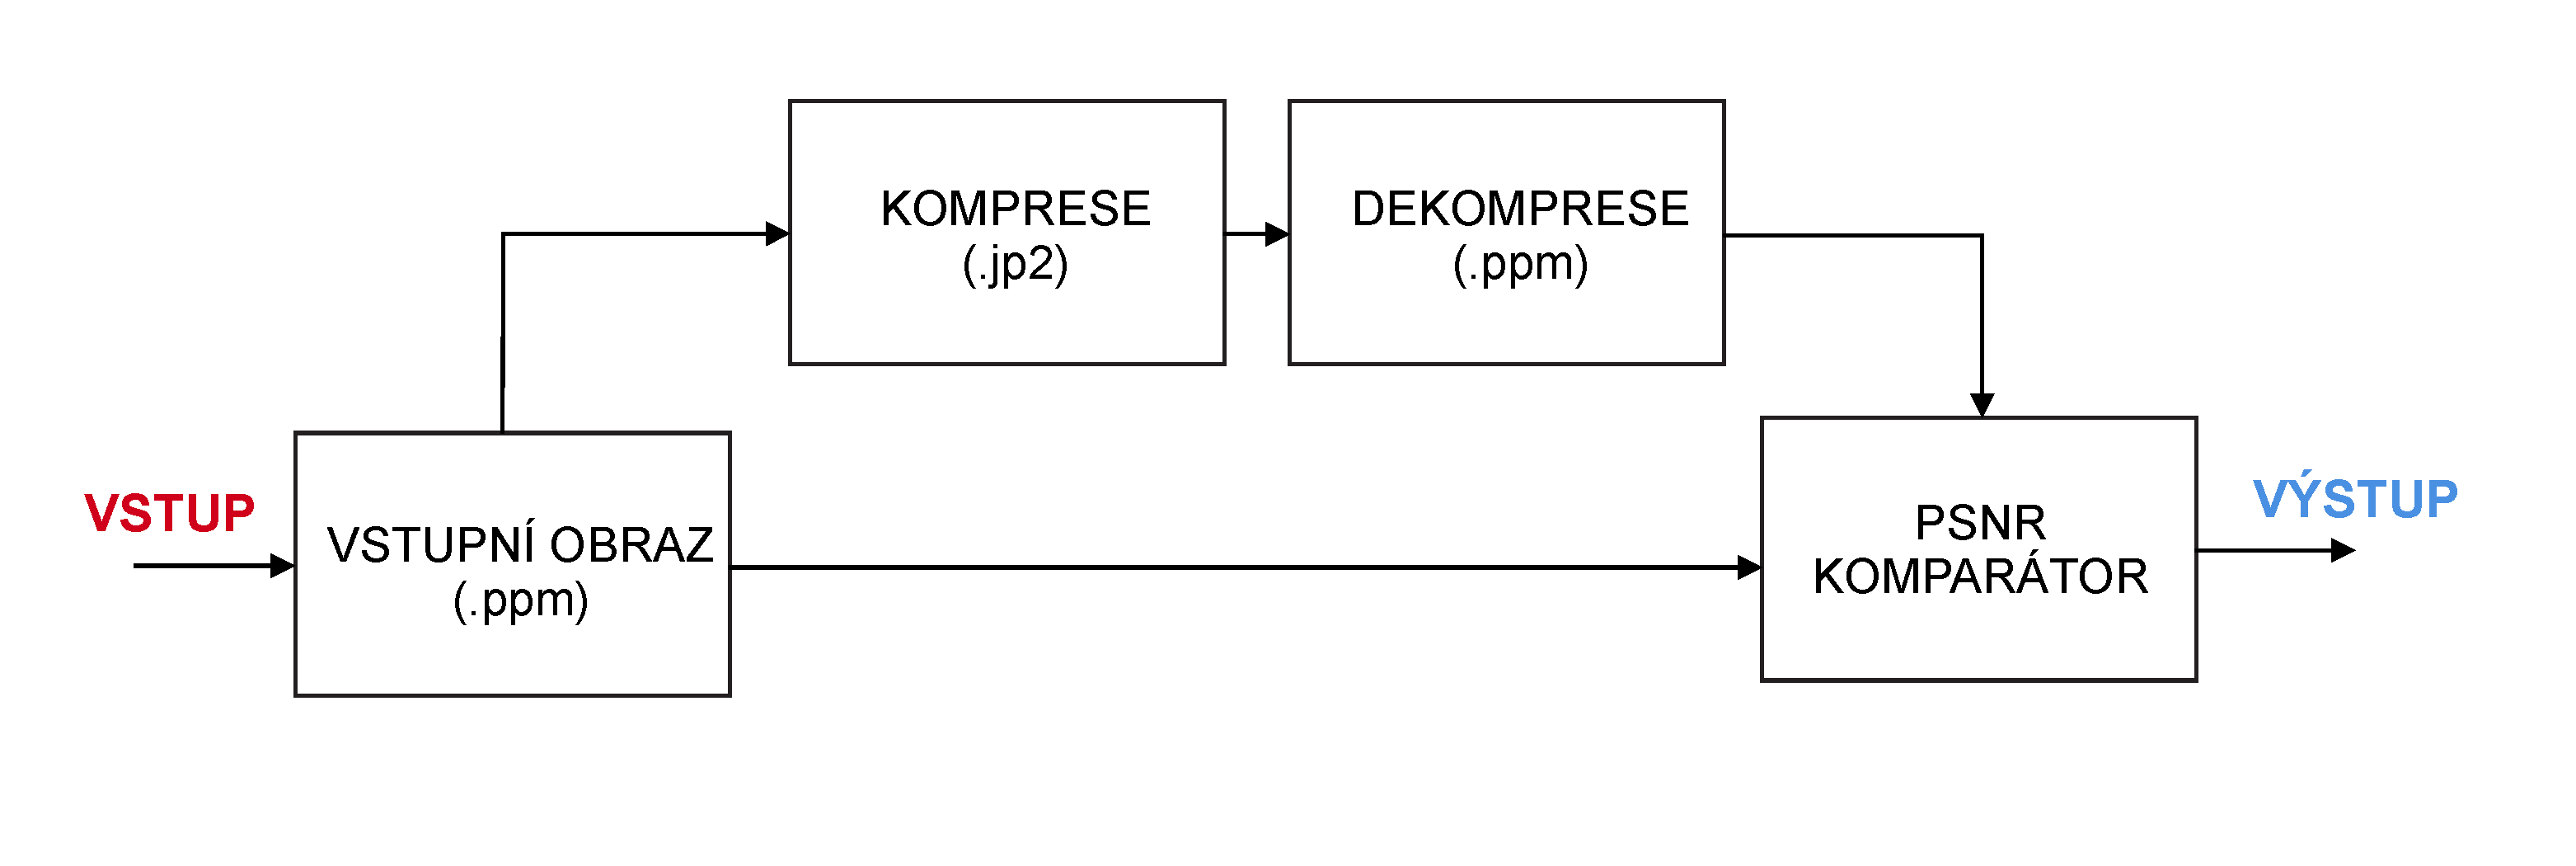
\includegraphics[width=16cm]{obrazky-figures/komparace.pdf}
  \caption{Blokové schéma komparace.}
  \label{retezec}
\end{figure}

\noindent Programová komparace dle PSNR je realizována následujícím způsobem. Vstupní data uložená jako .ppm/.pgm jsou zkomprimována do souboru .jp2, následně zpět dekomprimována do souboru .ppm/.pgm a porovnána s originálem.

\section{Další měřené veličiny}
V této práci kvalita není jedinou sledovanou veličinou.
\subsection*{Časová náročnost}
Přímý vliv na efektivitu uživatelské práce. Zpravidla není komprimován pouze jeden obrázek, ale často je nutno někam uložit sadu fotografií (např. z dovolené) nebo poslat větší množství scanovaných dat (technické výkresy). Tato veličina je přímo úměrná rychlosti pracovní stanice. Čas byl měřen utilitou \textit{usr/bin/time} a výstupem byl parametr \textit{real}. Tento parametr byl zvolen kvůli možnému běhu knihoven v režimu zpracování více vlákny. Parametr \textit{user} poskytuje pouze spotřebovaný čas jako ekvivalent jednoho vlákna.

\subsection*{Paměťová náročnost}
Nastaveními lze do určité míry ovlivnit i paměťovou náročnost. Tento výrok platí hlavně pro knihovnu OpenJPEG. Například volba velikosti dlaždice změní velikost zpracovávaného počtu dat. V případě dat o velikosti v řádech GB může nastat problém s nedostatkem paměti. Využití paměti bylo měřeno \textit{usr/bin/time -l} a výstupem byl parametr \textit{maximum resident set size}, který zaznamenává špičku paměti během celého běhu procesu. Jedná se tedy o nejhorší možný případ se kterým je nutno počítat.
\newpage
\section{Testovací data}
Dle zadání byly vytvořeny čtyři (dataset \textit{Bitonální} se ještě dělí na barevné a černobílé obrázky) datasety reprezentující možnosti a rozdíly mezi nastaveními.

\begin{table}[ht!]
  \centering
    \setlength{\tabcolsep}{3pt} % Default value: 6pt
    \renewcommand{\arraystretch}{1.15} % Default value: 1

    \begin{tabular}{|p{3.5cm}|p{3cm}|p{3cm}|p{3cm}|p{1.5cm}|}
      \hline
      \textbf{Typ} & \textbf{Velikost} & \textbf{Počet kanálů} & \textbf{Bitů na kanál} & \textbf{Počet} \\ 
      \hline

      Fotografie      & >100 MPx   & 3   & 8 & 110 \\ 
      Scany           & >80MPx     & 3   & 8   & 120 \\ 
      Mapy            & >75MPx     & 3   & 8   & 80 \\ 
      Bitonální RGB24 & >100MPx    & 3  & 8   & 110 \\ 
      Bitonální Gray8 & >100MPx    & 1  & 8   & 20 \\ 
      \hline
    \end{tabular}
    \caption{Základní informace o datasetech.} 
\end{table}

Pro statisticky významné měření obsahuje každý z datasetů alespoň 80 souborů. Jsou uloženy v formátu PPM/PGM ze specifikace Netpbm. Jedná se o formát obsahující surová data vhodně uložená k dalšímu zpracování.\\

\subsection*{Dataset \uv{Fotografie}}
Tento dataset slouží jako reference pro mnoho typů fotografií. Jedná se o soubor mnoha typů barevných fotografií (portréty, vesmírné, detaily, krajiny).

\subsection*{Dataset \uv{Scany}}
JPEG 2000 nabízí značné výhody při kompresi scanovaných dokumentů ať to jsou vrstvy kvality (dokáže nahradit mnoho adresářů s různými kvalitami jedním souborem) nebo speciální kompresní profily.

\subsection*{Dataset \uv{Mapy}}
Zpravidla s také jedná o scanované dokumenty, nicméně předchozí dataset jsou zpravidla obrazová data obsahující množinu textových znaků. Je možno nastavit silné úrovně komprese při zachování hodnoty informace (například pro OCR zpracování). Naopak u mapových podkladů - kdy množina tvarů není konečná, jako u textu, tzv. grafémy - je nutno zachovat preciznost obrazu. Jedná se o velice podrobné mapy s vysokým rozlišení, kde i malá míra zkreslení může mít velký dopad.

\subsection*{Dataset \uv{Bitonální}}
Bitonální obrazová data jsou ta, která obsahují pouze dva tóny (dvě barvy). Jedná o experimentální měření, protože tento typ dat není běžně používán. Jsou ovšem velmi zajímavé z hlediska nastavení kompresního řetězce, jelikož se jedná o relativně exotický obrazový materiál, u kterého lze po vhodném nastavení očekávat zlepšení. Část datasetu slouží k testování vstupní dat v úrovních šedi (Gray8).

\vspace{3.5cm}
\begin{figure}[hbt!]
  \centering
  \hspace*{-0.75cm}
  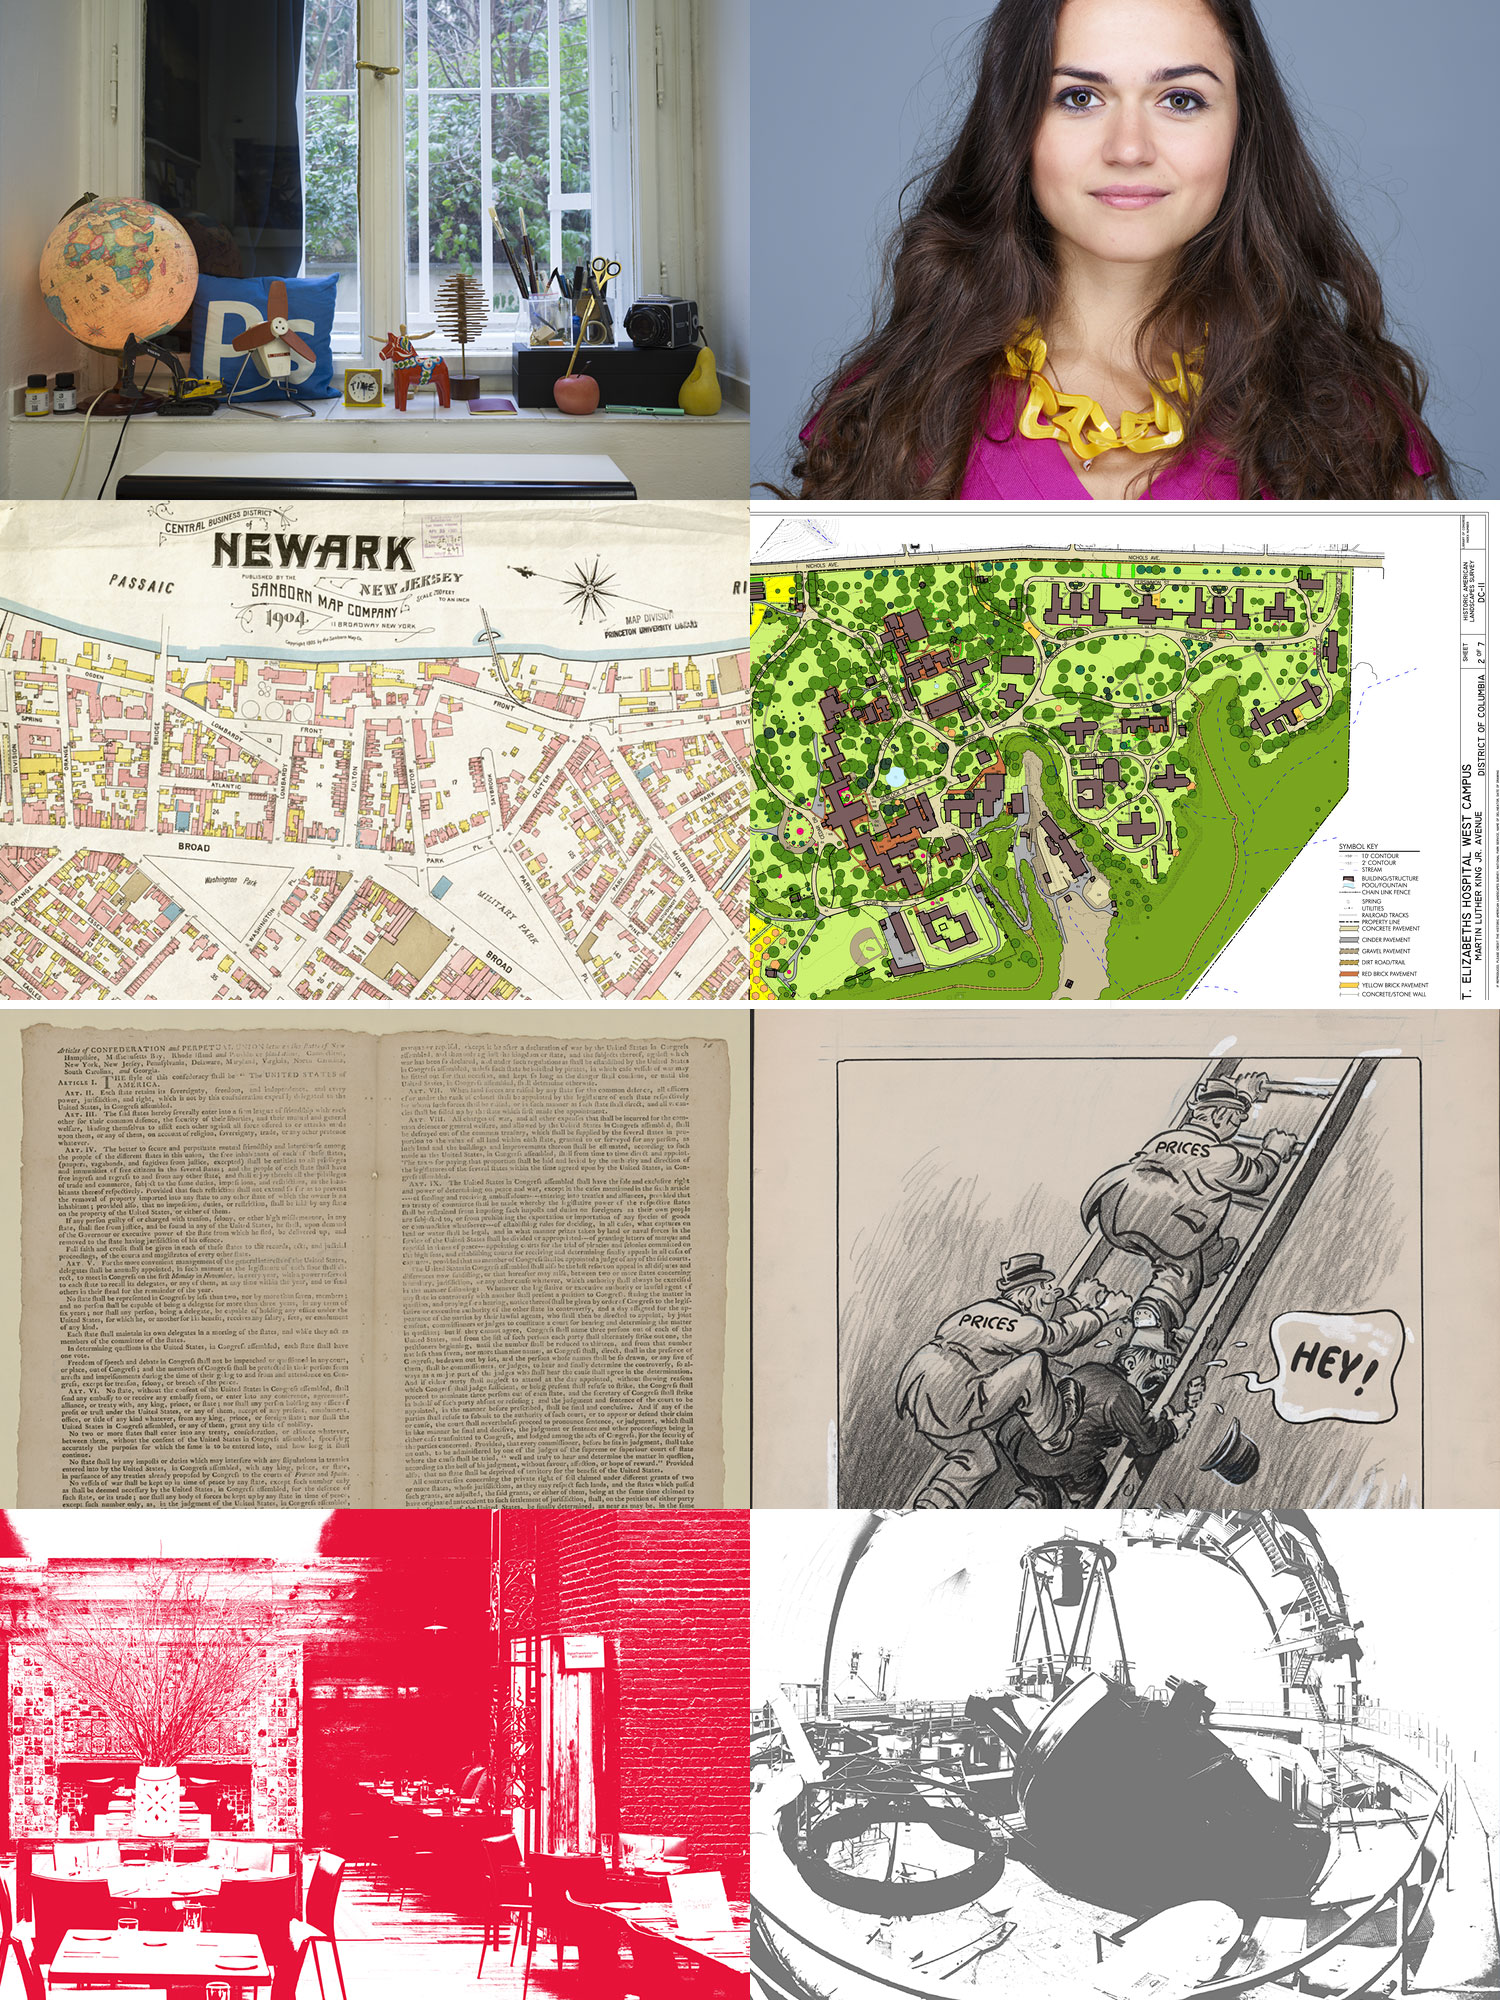
\includegraphics[width=16cm]{obrazky-figures/fotky.jpg}
  \caption{Náhled zpracovávaných datasetů.}
  \label{keepCalm}
\end{figure}


\clearpage
\newpage
\section{Implementace} 
Implementace testovacího nástroje proběhla v jazyce Python verze 3 s využitím knihovny numpy pro matematické výpočty a nerelační databází MongoDB pro průběžné ukládání výsledků. Byl kladen velký důraz rozšiřitelnost a uživatelský komfort. Průběžné ukládání informací o testech slouží pro účely zpřesňování výsledků a vykreslování grafů. Jako implementace formátu JPEG 2000 byly použity dvě knihovny - Kakadu \cite{kakadu_docs} a OpenJPEG \cite{open_docs}. Každá z knihoven přistupuje k dané problematice jinak, hlavně kvůli tržnímu statutu, kdy Kakadu plní roli komerčního nástroje pro velké instituce a OpenJPEG je nejpoužívanější implementace s volně dostupným zdrojovým kódem. Z hlediska pokrytí standardu má jasně navrch Kakadu, které umožňuje pokročilejší práci s parametry nastavení. Nutno dodat, že ani jedna z knihoven plně nepokrývá ani první část standardu, na druhou stranu Kakadu obsahuje naprostou většinu podstatných věcí (např. chybí markery PPM/PLT). Vzhledem k použití obou knihoven při testování odpadá možnost vyšetřovat určité parametry simultánně - hlavně u OpenJPEG - který některé nastavení neimplementuje nebo ignoruje.

\subsection*{Testovací nástroj}
Testovací nástroj je spouštěn z příkazové řádky v třech variantách. Před každým testem - a po určité uživatelem nastavitelné době - je nejdříve nutno projít vybranou složku a zjistit informace o všech souborech. Mezi nejdůležitější informace patří rozlišení obrazu, počet kanálů a bitová hloubka. Tyto informace umožňují efektivně počítat kompresní poměr a pomáhají s nastavením kompresního řetězce. Po úspěšném získání jsou výsledky testování uloženy do databáze. Nástroj funguje pouze nad obrazovým materiálem ve formátu .ppm pro tří složkové a .pgm pro jednosložkové obrázky. Nejdůležitější variantou spuštění je testování. Jak již bylo zmíněno v předešlé sekci, každé testovací sezení disponuje svým předpisem. Všechny jsou uloženy ve formátu .json pro snadnější strojové zpracování. V jednom souboru se může nacházet více sezení. 


\begin{figure}[hbt!]
  \hspace*{-0.5cm}
  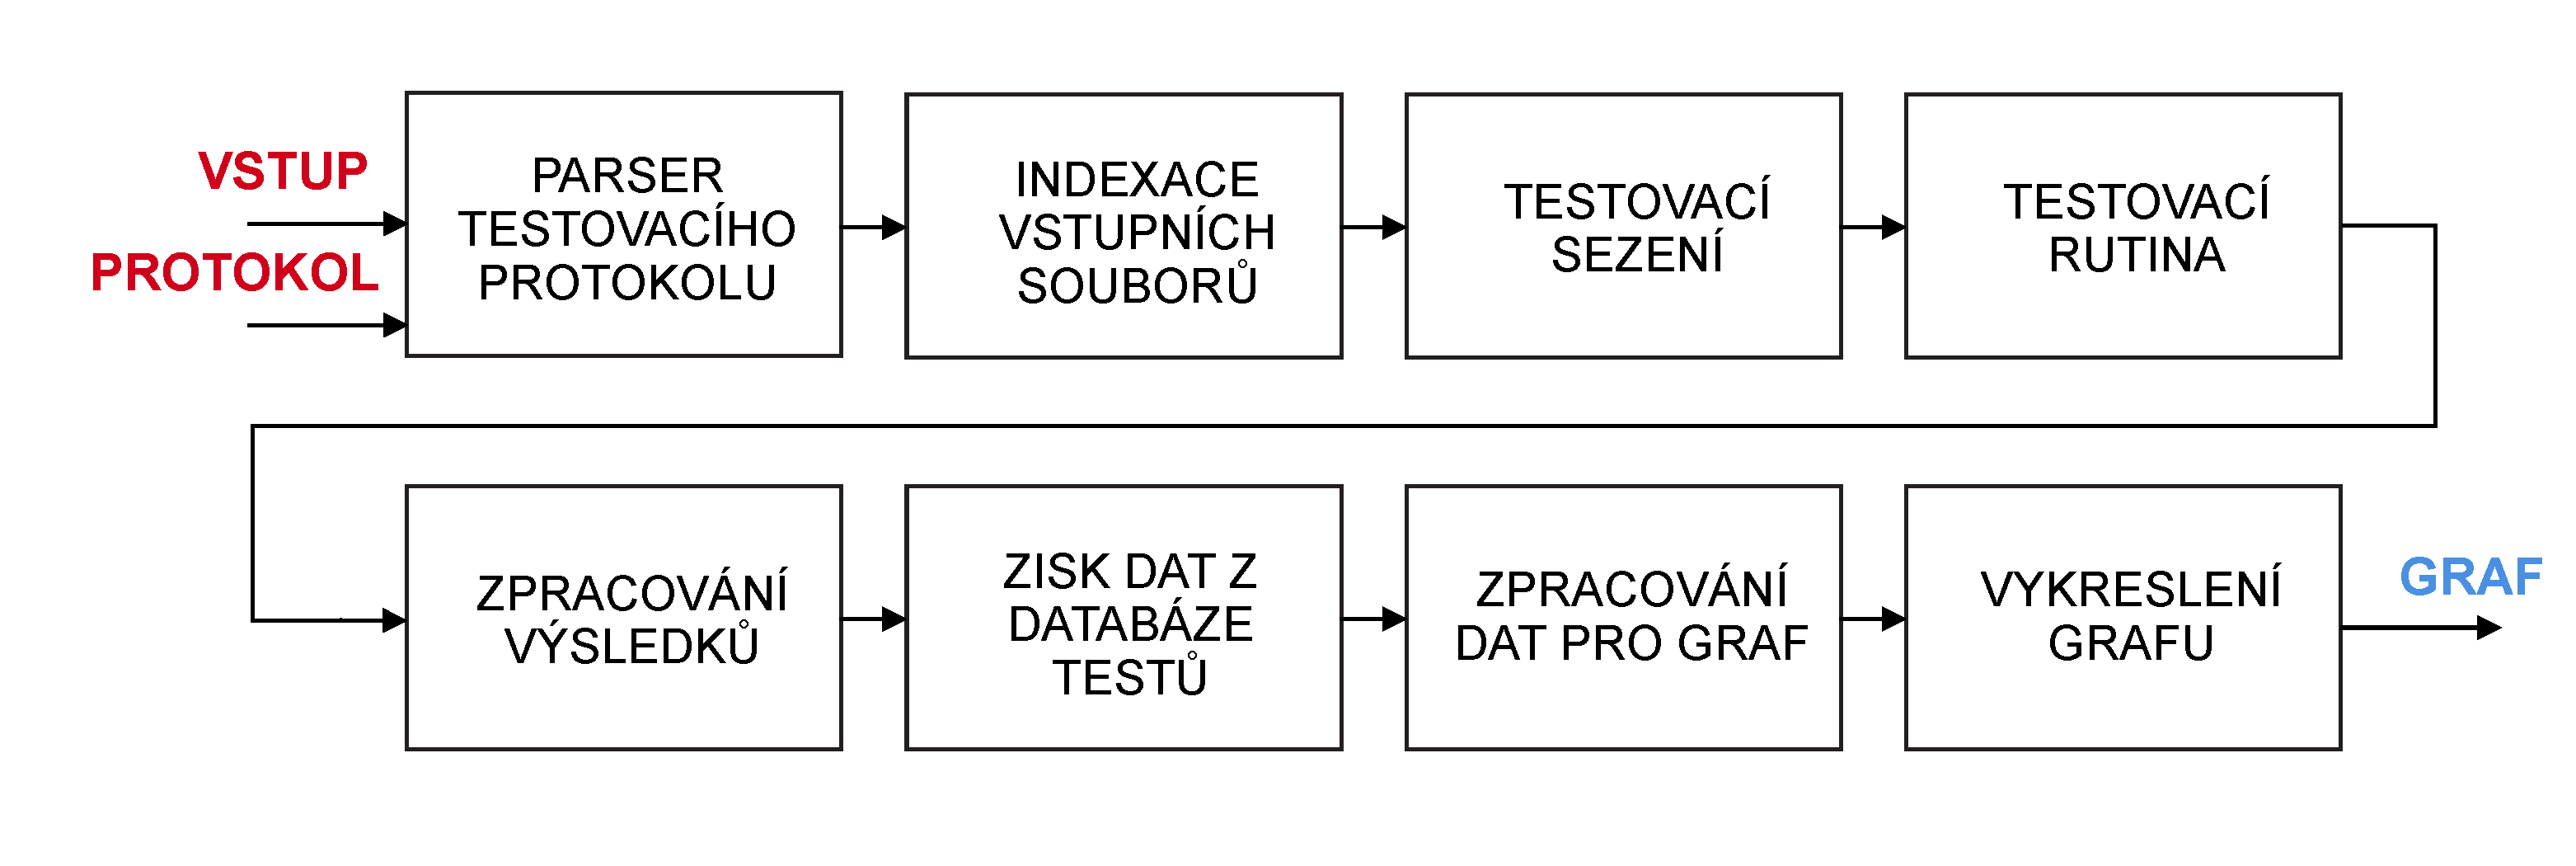
\includegraphics[width=16cm]{obrazky-figures/schema.pdf}
  \caption{Blokové schéma testovacího nástroje.}
  \label{retezec}
\end{figure}

\clearpage

\begin{lstlisting}
{
    "type"      : "approximation",
    "files"     : {}
    "dir"       : "path",
    "drivers"   : ["drivers"],
    "routines"  : {
        "compress": {   
            "criterion"     : {
                "type"  : "psnr",
                "value" : [opt1...]
            },
            "testing_param" : {
                "flag"  : "tiles",
                "opts"  : [opt1...]
            },
            "params"        : {}
        },
        "decompress": {
            "testing_param" : {},
            "params"        : {}
        }
    }
}
\end{lstlisting}

Základní struktura předpisu testovacího sezení je relativně jednoduchá. Nejprve je nutno zvolit druh. Ten určuje počet opakování testu pro zajištění statistické věrohodnosti vyšetřených výsledků, hlavně časových a paměťových nároků. Existují dva druhy testování: aproximační a koncové. Pokud by jediné kritérium vyšetřování komprese byla bitová hloubky, stačilo by pouze koncové testování s dostatečným počtem opakování. Když je jako kritérium PSNR, nelze dopředu jednoznačně určit jakému PSNR odpovídá konkrétní bitová hloubka. Lze přibližně určit interval, kde se nachází, avšak pro dosažení přesnosti aproximace (zvolena na dvě desetinná místa) je nutno každý soubor - a každou jeho variantu - několikrát prohnat celým řetězcem zpracování. Tato problematika klade značné nároky na rychlost určení odhadu a zvolenou metodu aproximace. Byl kladen velký důraz na kvalitu implementace, jelikož zpracovávané souboru velmi často dosahují značných velikostí, které znesnadňují efektivní algoritmizaci problému. Proběhly pokusy se strojovým učením, které byly ovšem záhy opuštěny z důvodu značného zesložitění programu s nevalnými výsledky v časové doméně. Možnost zjednodušení se také jevila při zmenšení souborů (řádově jednotky megapixelů) a jejich následné vyšetření pomocí triviálních algoritmů jako je např. bisekce intervalu. Tento přístup dosahoval velmi dobrých výkonů, avšak křivka kvality není přesně škálovatelná - hlavně u atypický dat. Určení intervalu obsahujícího řešení bylo velmi rychlé. Kromě zmenšení obrazu, jelikož se jedná o výpočetně náročnou operaci, kterou lze provést ale před testováním, nicméně úvodní náklady na testování neúměrně vzrostou. S vymezeným intervalem stačilo pouze najít koeficient zvětšení obrazu a kvality, což bylo realizováno výpočtem rozdílů kvalit na obou koncích intervalu původního i zmenšeného souboru. Při testování toho přístupu se zvolenou přesností na jedno desetinné místo algoritmus vykazoval mnohem lepší výsledky než referenční řešení (bisekce intervalu). Jakmile byla zvolena přesnost vyšších řádů výhoda počátečního určení intervalu a následné lepší aproximace byla smazána, jelikož dramaticky vzrostl počet kompresí původního souboru na úkor zmenšeného. Když se připočte nutnost ošetření mnoha extrémních stavů byl tento přístup také opuštěn. Výsledkem aproximační fáze je v obou případech bitová hloubka, která u PSNR odpovídá zvolenému kritériu s určenou přesností. Následuje koncové testování, které si z databáze načte aproximační výsledky a na jejich základě testuje již vyšetřené kritérium s určitým počtem opakování pro zajištění statistické přesnosti a odstranění šumu. Tyto výsledky již slouží jako data ke grafům.\\
Po výběru druhu je třeba zajistit práci se soubory. Soubory je lze filtrovat dle jména, omezit jejich počet nebo některé explicitně z testování vyjmout. Jelikož byl testovací nástroj zamýšlen jako plně rozšiřitelný pro další knihovny, je uživateli nabídnuta volba použitých knihoven. Následuje nastavení komprese a dekomprese. U obou jsou parametry děleny na dvě množiny. První z nich jsou pevné, které se nemění během celého trvání testování. Druhá obsahuje vyšetřovaný parametr a hodnoty jež nabývá. Počet záznamů v databázi odpovídá počtu vyšetřovaných hodnot. Tímto fáze testování končí, následuje zpracování dat a vykreslení grafu. Opět se jedná o netriviální práci, jelikož existují dvě kritéria, jenž vyžadují odlišené zpracování a sekundární data k vykreslení (časová a paměťová náročnost). Vykreslovaní nástroj umožňuje kombinovat více testovací sezení, dokonce i s rozdílnými vyšetřovanými parametry při zaručení vzájemné kompatibility pevný parametrů. V neposlední řadě nabízí uživateli volbu rozsahů, typů a popisu grafů.

% \todo{Blokove schema testeru}
% \todo{Popis testeru}
% \todo{CPU graf}

% \begin{figure}[hbt]
%   \centering
%   \includegraphics[width=14cm]{obrazky-figures/cores.png}
%   \caption{Resident Set Size (RSS), maximální pamět využitá pro kompresi. Kakadu roste pouze minimálně, evidentně zpracovává velice podobné bloky bez ohlednu na rozlišení obrázku. OpenJPEG implicitně načte celý obrázek do paměti, což v extrémních případech může být problém.}
%   \label{keepCalm}
% \end{figure}
% \clearpage


\chapter{Analýza nastavení formátu}
\label{analyza}
V této kapitole jsou rozebrány možnosti komprese (ať již ztrátové či bezeztrátové) vzhledem k možnostem parametrů knihoven Kakadu a OpenJPEG implementující formát JPEG 2000. Technická stránka vyšetřování je osvětlena v předchozí kapitole. Byla zadána množina zkoumaných parametrů k vyšetření. Nejprve jsou demonstrovány používané profily a pro každý z pěti datasetů je zvolen jeden jako referenční. Každý parametr má svůj obor hodnot. Konkrétní nastavení parametru dle vybraného referenčního profilu je okomentováno, pokud je jím definován. Testováním je ověřena jeho vhodnost, případně slouží jako základ pro doporučení jiné volby. Pokud to knihovna dovolí, budou parametry vyšetřovány u obou zástupců, stejně tak jako časová a paměťová náročnost. Aby nebyl čtenář zatěžován množstvím nadbytečných grafů, které ilustrují stejný jev, ne vždy budou demonstrovány všechny hodnoty. Stane se tak pouze v případě, když mezi nimi bude dostatečný rozdíl či bude potřeba poukázat na konkrétní jev u dané knihovny/datasetu nebo profilu.  
V předchozích kapitole bylo vysvětleno v čem je aproximace k určitému PSNR vhodná, nicméně když je odhlédnuto od implementační a časové náročnosti nachází se zde ještě jeden problém. Parametr je vyšetřen pouze v jednom bodě kvalitativní stupnice - resp. ve dvou, pro ztrátovou a bezeztrátovou - ale obě knihovny škálují s změnami kvality symetricky, proto tento přístup v naprosté většině případů dostačuje. Tam, kde záhodno ukázat průběh jevu na větším intervalu bude místo PSNR využita bitová hloubka jako kritérium. Některé testy se liší typem grafům. Cílem je ukázat spojitost veličiny, kdy např. převod barevného prostoru lze zapnout či vypnout, ale velikost dlaždice může být prakticky jakákoliv bez ohledu na poměr a velikost (samozřejmě respektující velikost vstupního obrazu). Nakonec jsou zhodnoceny všechny dílčí výsledky měření, je poukázáno na zajímavé jevy a vydána sada doporučení pro práci s daným datasetem a knihovnou. Posloupnost vyšetřovaných parametrů není náhodná. Každý následující test využívá doporučené nastavení z předchozího testu.

\newpage
\subsection*{Existující profily JPEG 2000}
Ačkoliv se JPEG 2000 na spotřebitelském trhu neuchytil, tak jak si autoři představovali, knihovny a archivační instituce po celém světě jej hojně používají. Většina zde zmíněných profilu pochází z těchto zdrojů. Existují v relativně velké množství, nicméně drtivá většina z nich je velmi obecně zaměřena (fotografie či manuskripty) pro ztrátovou kompresi.  Jak se v průběhu vyšetřování ukáže, mnohokrát se vyplatí pro určitý dataset věnovat úsilí při sestavování specifického profilu.\\

\begin{table}[ht!]
\small
    \setlength{\tabcolsep}{3pt} % Default value: 6pt
    \renewcommand{\arraystretch}{1.5} % Default value: 1
    \begin{tabular}{|p{4cm}||p{2.5cm}|p{2.5cm}|p{2.5cm}|p{2.5cm}|}
      \hline
      \textbf{Parametr}             & \textbf{Fotografie}          & \textbf{Mapy}      & \textbf{Scany}    & \textbf{Bitonální} \\ 
      \hline
      kompresní poměr               & 6:1                          & 8:1 až 10:1        & neuvedeno         & 10:1 \\ 
      typ komprese                  & ztrátová                     & ztrátová           & ztrátová          & ztrátová \\ 
      dlaždice                      & 1024x1024                    & 1024x1024          & NE                & NE \\ 
      pořadí přenosu                & RLCP                         & RPCL               & RPCL              & RPCL \\ 
      dekompoziční úrovně           & 5                            & 5 až 6             & 6                 & 7 \\ 
      vrstvy kvality                & 8                            & 12                 & ANO               & 7 \\ 
      ROI                           & NE                           & NE                 & NE                & NE \\ 
      code-block                    & 64x64                        & 64x64              & 64x64             & 64x64 \\ 
      profily EBCOT                 & NE                           & Bypass             & NE                & NE \\ 
      \hline
    \end{tabular}
    \caption{Profily ztrátové komprese. Jako zdroje těchto profilů slouží podklady Národní digitální knihovny \cite{ndk}, British Library \cite{bl} a Bibliotheca Alexandrina \cite{al}.} 
\end{table}

\begin{table}[ht!]
\small
    \setlength{\tabcolsep}{3pt} % Default value: 6pt
    \renewcommand{\arraystretch}{1.5} % Default value: 1
    \begin{tabular}{|p{4.4cm}||p{5cm}|p{5cm}|}
      \hline
      \textbf{Parametr}             & \textbf{Fotografie a Bitonální}          & \textbf{Mapy a Scany} \\      
      \hline
      kompresní poměr               & 2:1                          & 3:1                \\ 
      typ komprese                  & bezeztrátová                 & bezeztrátová       \\ 
      dlaždice                      & 4096x4096                    & NE                 \\ 
      pořadí přenosu                & RPCL                         & RPCL               \\ 
      dekompoziční úrovně           & 5 až 6                       & 6                  \\ 
      vrstvy kvality                & 1                            & 6                  \\ 
      ROI                           & NE                           & NE                 \\ 
      code-block                    & 64x64                        & 32x32              \\ 
      profily EBCOT                 & NE                           & neuvedeno          \\ 
      \hline
    \end{tabular}
    \caption{Profily bezeztrátové komprese. Jako zdroje těchto profilů slouží podklady Národní digitální knihovny \cite{ndk} a Library of Congress \cite{cong}.} 
\end{table}


\newpage
\section{Porovnání formátů a testovací kritérium}

% =======================================================================
% -----------------------------------------------------------------------
%
% Criterion
%
% -----------------------------------------------------------------------
% =======================================================================
Před samotným testováním je vhodné demonstrovat, kde se nachází obor hodnot sloužících jako kvalitativní nastavení komprese, jaké výkony komprese lze očekávat a jak moc se liší kompresní výkon mezi JPEG 2000 a jeho předchůdcem. Pro testování se zvoleným kritériem PSNR ztrátové komprese je nutno určit hodnotu, která bude reprezentativní napříč datasety. Bitová hloubka vykazuje nejzajímavější hodnoty z pohledku komprese kolem kvality \textbf{35 dB}. Tato hodnota bude použita jako univerzální kritérium PSNR při testování ztrátové komprese.
\begin{figure}[hbt!]
  \centering
  \hspace*{-0.5cm}
  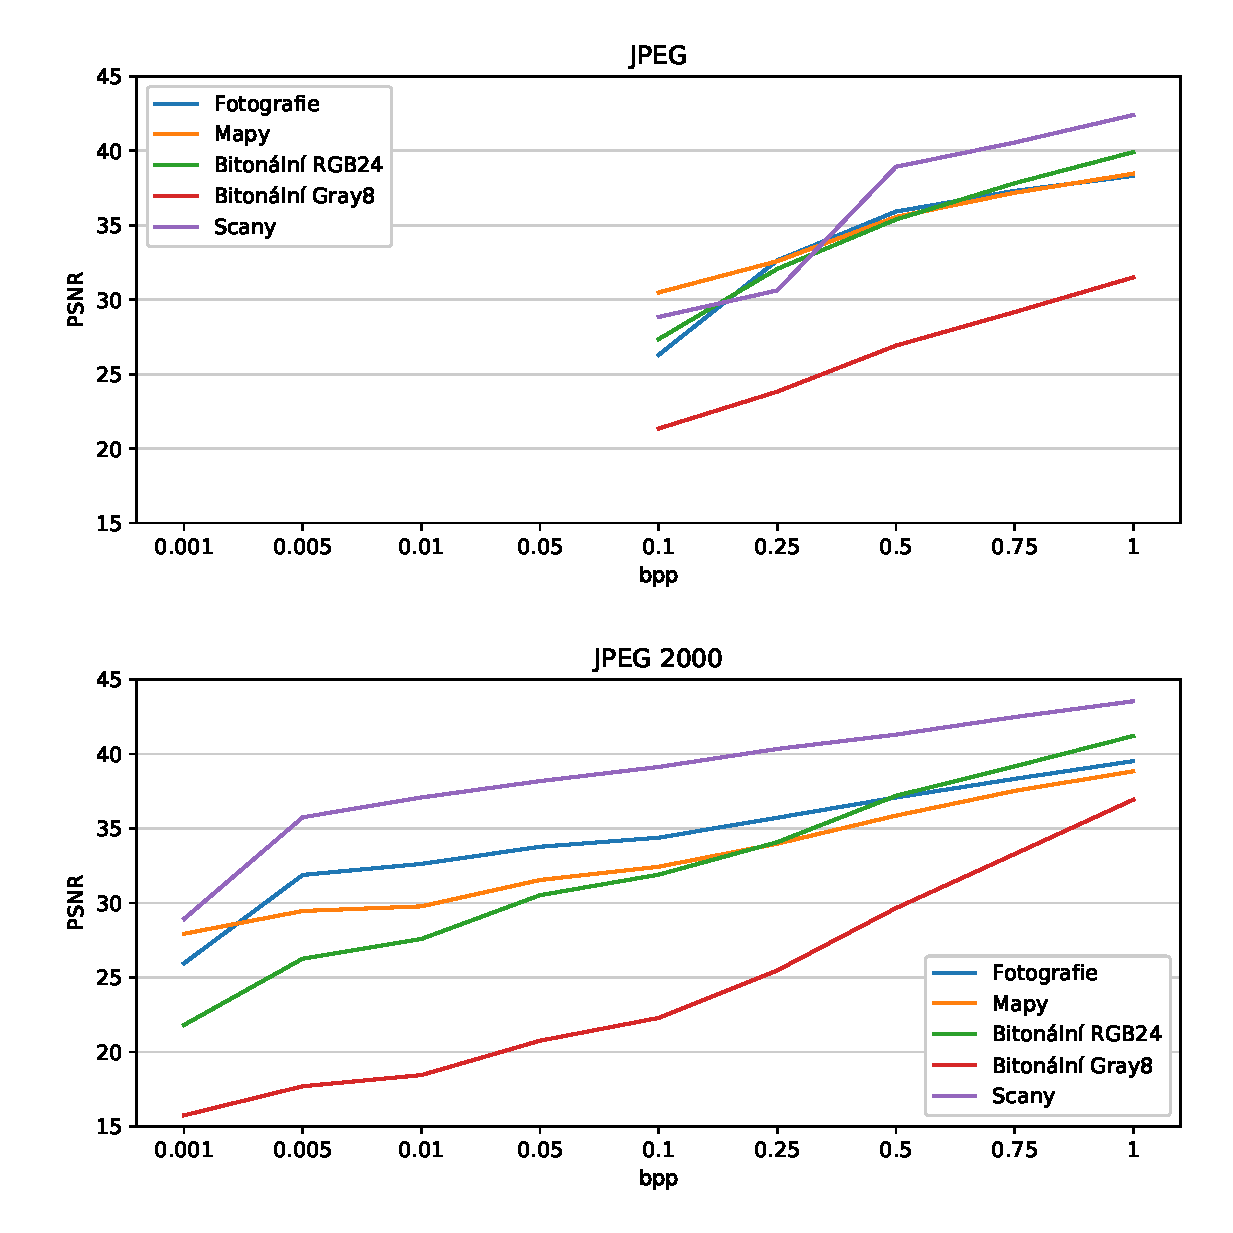
\includegraphics[width=16cm]{obrazky-figures/porovnani.eps}
  \caption{Porovnání kompresních výkonů. Pro kompresi dle formátu JPEG byl použit nástroj Imagemagick s kompresní utilitou \textit{convert}.}
\end{figure}
\clearpage

\noindent Při prvním pohledu do grafů je očividná jedna věc. JPEG nedisponuje možností zvolit menší hodnotu bitové hloubky než 0.1 bpp. Zároveň nedisponuje příliš flexibilním způsobem nastavování kvality. Kvalitu lze ovlivnit pouze volbou nastavení kvantizační matice, a to v intervalu <1,100> s krokem v celých celých číslech. Nelze přesně zadat zvolenou kvalitu, je nutno ji dopočítat aproximačním způsobem. V tomto testu byla dosažena přesnost aproximace na dvě desetinná místa, která pro ilustraci dostačuje.
Z mnoha důvodů - DCT transformace, kódování - se nelze ani zdaleka přiblížit efektivitě komprese JPEG 2000. Průměrný rozdíl v kvalitě komprese při stejném bpp dosahuje \textbf{12.43\%}. Při menších bpp je rozdíl ještě markantnější, kdy v intervalu <0.1,0.5> bpp je rozdíl nezanedbatelných \textbf{26.74\%}, což je zprůměrovaná hodnota pro všechny datasety. Největší rozdíl v tomto intervalu vykazuje dataset \uv{Scany} s více než o třetinu lepším kompresím výkonem (\textbf{35.81\%}). Vzhledem k neschopnosti JPEG se neprojevily plné schopnosti jeho nástupce. JPEG 2000 exceluje při velmi malých bitových hloubkách. Např. u datasetu \uv{Fotografie} odpovídá stejné PSNR jako u JPEG osmdesátinásobně menší bitové hloubce. Spolu s pořadí přenosu lze docílit již při opravdu velkých kompresních poměrech alespoň náhledové kvality použitelné např. na webu.

\begin{figure}[hbt!]
  \centering
  \hspace*{-0.75cm}
  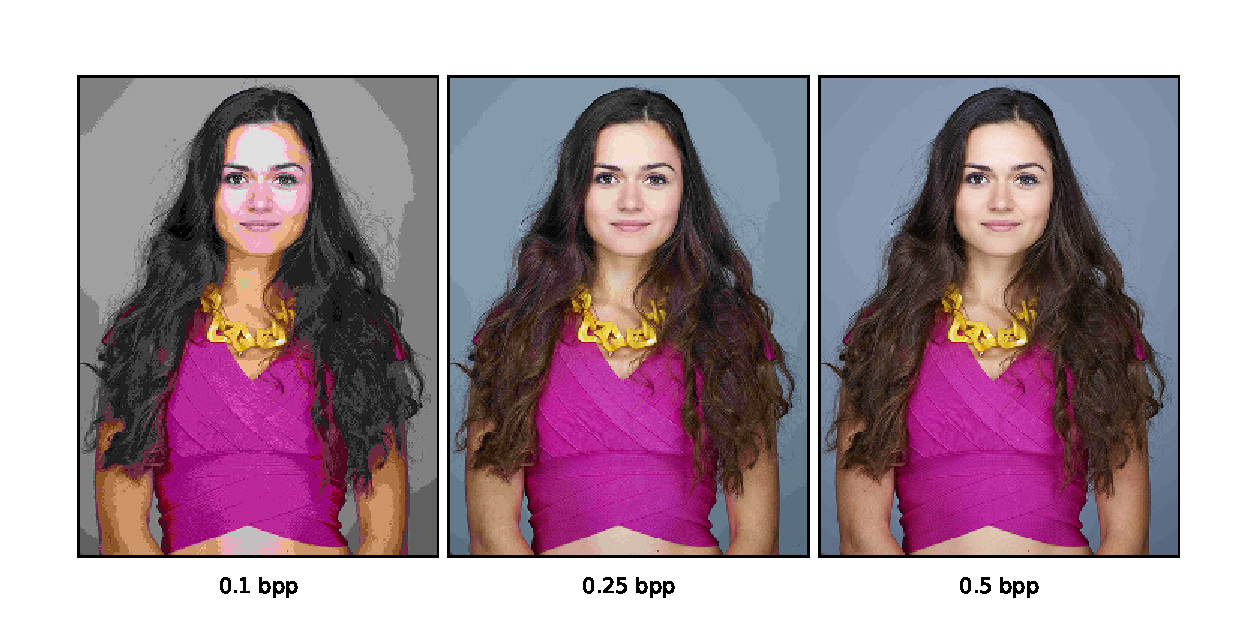
\includegraphics[width=16cm]{obrazky-figures/odhad/fotky_kvalita_jpeg_odhad.eps}
  \caption{Průběh kvality JPEG.}
\end{figure}

\noindent Kompresní artefakty se malé míře objevují již při 0.5 bpp. Obraz je však stále dostatečně kvalitní i v plném rozlišení. Poloviční bpp vykazuje známky začínající posterizace, která je způsobena malým tonálním rozsahem. Minimální možná kvalita vykazuje značnou posterizaci. Takto zkomprimovaný obraz může sloužit maximálně jako malý náhled.

\clearpage
\begin{figure}[hbt!]
  \centering
  \hspace*{-0.75cm}
  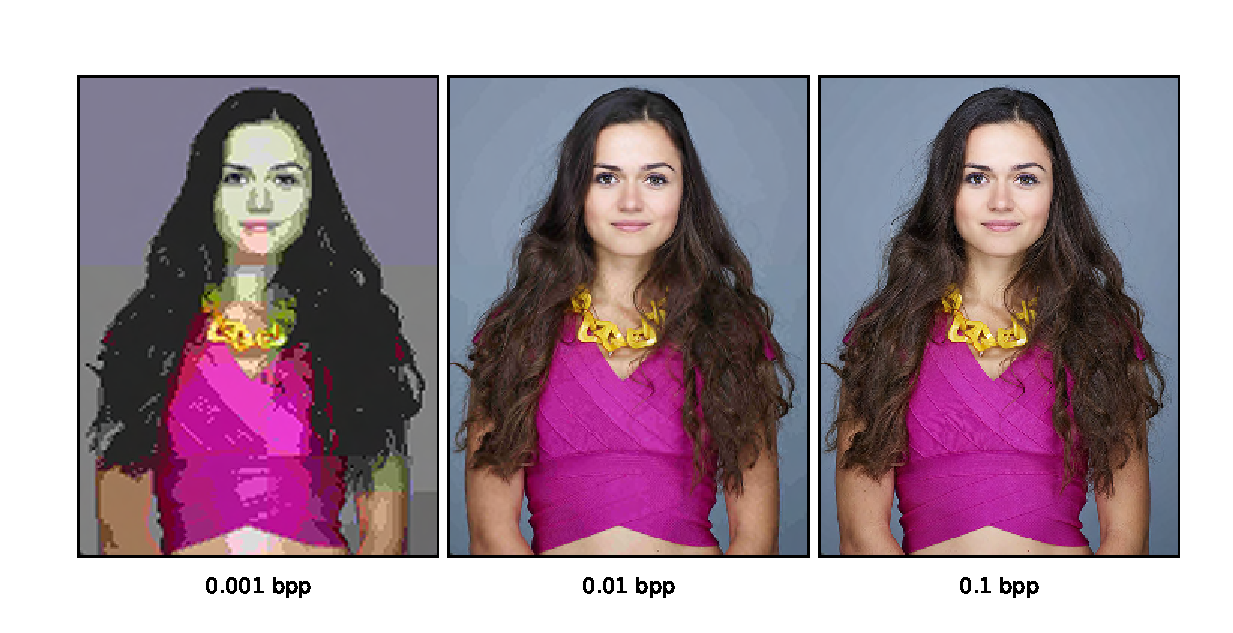
\includegraphics[width=16cm]{obrazky-figures/odhad/fotky_kvalita_odhad.eps}
  \caption{Průběh kvality JPEG 2000.}
\end{figure}

\noindent Tam, kde JPEG končí s nejmenším možným nastavitelnou bitovou hloubkou JPEG 2000 začíná. 0.1 bpp znamená velmi kvalitní obraz, který lze použít i při plném rozlišení. Desetinásobně zmenšená bitová hloubka stále věrohodně reprezentuje barevné spektrum bez známek kompresních artefaktů Rozumné minimum u JPEG 2000 se pohybuje hranici 0.001 bpp, kde je už silně znát velký kompresní poměr, obraz trpí značnou posterizací a je - i bez použití dlaždicového mechanismu - znatelné blokové dělení.\\
Časové a paměťové nároky jsou často udávány jako jedna z velkých nevýhod JPEG 2000. U první jmenované se neprokázal velký rozdíl, průměrně \textbf{9.71\%}. Paměťové nároky ovšem můžou hrát roli při výběru formátu, jelikož průměrná hodnota maximální využité operační paměti při zpracování vzrostla u JPEG 2000 o \textbf{27.44\%}. Tento fakt ovlivňuje mnoho mechanismů, které budou probrány v dalších sekcí (např. velikost dlaždice). Celkově lze JPEG 2000 doporučit. Dosahuje násobně lepších kompresní výkonů - hlavně u velkých kompresních poměrů - při celkovém patnáctiprocentním zvýšení režie. 

\clearpage
\newpage
\section{Vyšetřování parametrů}
Tato sekce se zaměřuje testování parametrů pro ztrátovou i bezeztrátovou kompresi. Měřítka grafů jsou vzájemně porovnatelná dle typů komprese.
% =======================================================================
% -----------------------------------------------------------------------
%
% Color transform
%
% -----------------------------------------------------------------------
% =======================================================================
\subsection*{Převod barevného prostoru}
Jedná se o první krok, který je nutno provést při zpracování vstupních dat. V praxi používá dvou cest, ICT a RCT pro ztrátovou, resp. bezeztrátovou kompresi. Všechny datasety jsou uloženy v RGB prostoru - kromě \uv{Bitonální Gray8}, který v tomto testu nemá smysl vyšetřovat, jelikož není reprezentovaný ve třech, ale pouze v jedné složce - komponentě, podle terminologie JPEG 2000. Profily se tímto parametrem nezabývají, nelze využít referenčního nastavení. Podvzorkování je v při tomto testu vypnuto.
\newline

\begin{figure}[hbt!]
  \centering
  \hspace*{-0.75cm}
  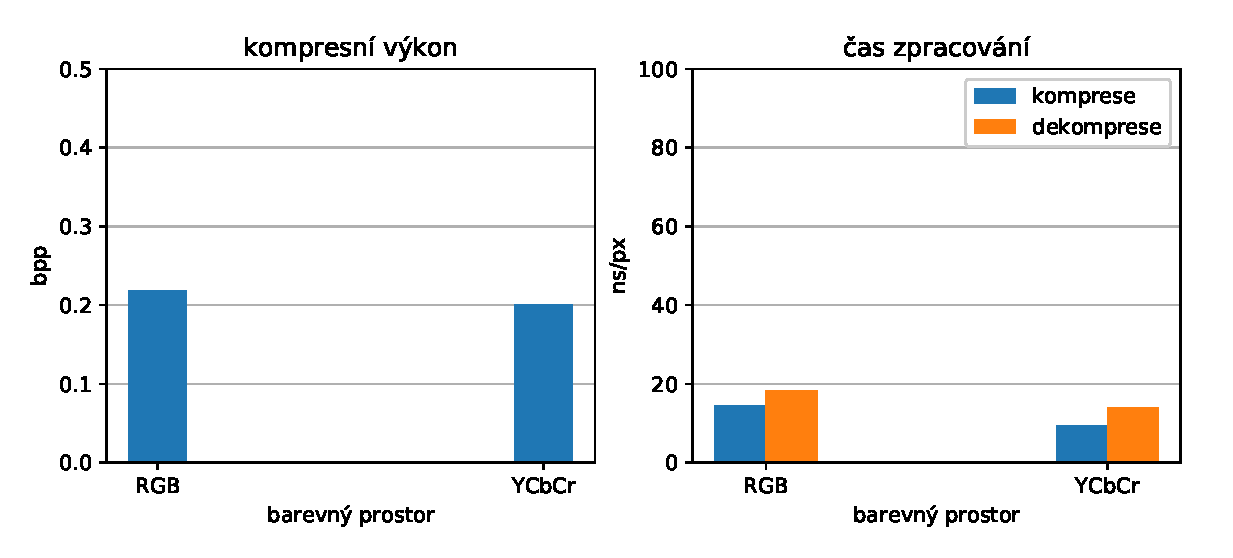
\includegraphics[width=16cm]{obrazky-figures/rgb_ycrcb/fotky_rgb_ycrcb.eps}
  \caption{Převod barevného prostoru - ztrátově.}
\end{figure}

\indent Nepoužití převodu barevného prostoru napříč datasety zvětší výsledný soubor \textbf{9.78\%} a zpomalí zpracování souboru o \textbf{26.77\%}. Pro ztrátovou kompresi lze jednoznačně doporučit převod barevného prostoru.
\clearpage
\begin{figure}[hbt!]
  \centering
  \hspace*{-0.75cm}
  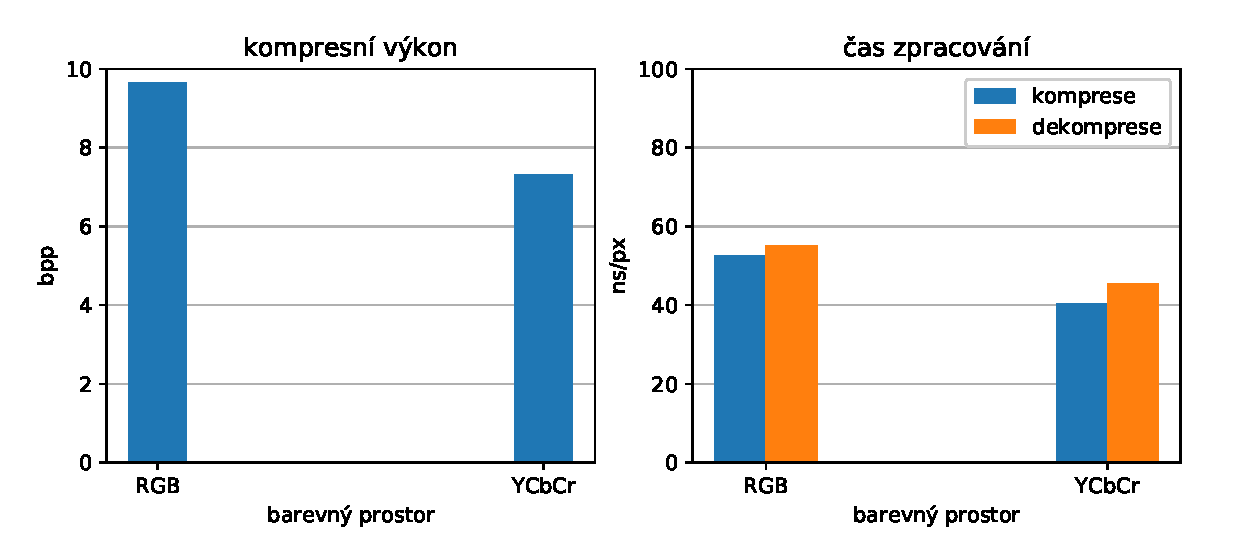
\includegraphics[width=16cm]{obrazky-figures/rgb_ycrcb/fotky_full_rgb_ycrcb.eps}
  \caption{Převod barevného prostoru - bezeztrátově.}
\end{figure}

\indent Nepoužití převodu barevného prostoru napříč datasety zvětší výsledný soubor \textbf{31.74\%} a zpomalí zpracování souboru o \textbf{14.98\%}. Pro bezeztrátovou kompresi lze jednoznačně doporučit převod barevného prostoru. Jasně se ukázalo, že nepoužití převodu vede k u obou typů kompresí ke zhoršení kompresního výkonu.

% =======================================================================
% -----------------------------------------------------------------------
%
% Tiles
%
% -----------------------------------------------------------------------
% =======================================================================
\newpage
\subsection*{Dlaždice}
Jeden ze základních parametrů nastavení umožnující plné využití formátu JPEG 2000. Obraz je rozdělen na části, které jsou samostatně zpracovávány. Tento krok dovoluje aplikovat ostatní parametry nikoliv na celý obraz, avšak pouze na dlaždici. V terminologii JPEG 2000 nazýváno \textit{Tile-parts}. Typickým příkladem jsou tzv. \textit{compound images}, které obsahují více typů obrazových dat v jednom obraze. Strojové vyšetřování tohoto nastavení je obtížné, jelikož se musí jednat obraz, který obsahuje přesně definované části s rozdílným obsahem.  Každá dlaždice má určitou režii - násobená volbou precinctu, při testování nepoužity - a při použití velmi malých dlaždic (128x128 px, 64x64 px) vznikají blokové kompresní artefakty. Velikosti dlaždic jsou při tomto testu čtvercové, ale lze zvolit libovolný poměr stran.

\begin{figure}[hbt!]
  \centering
  \hspace*{-0.75cm}
  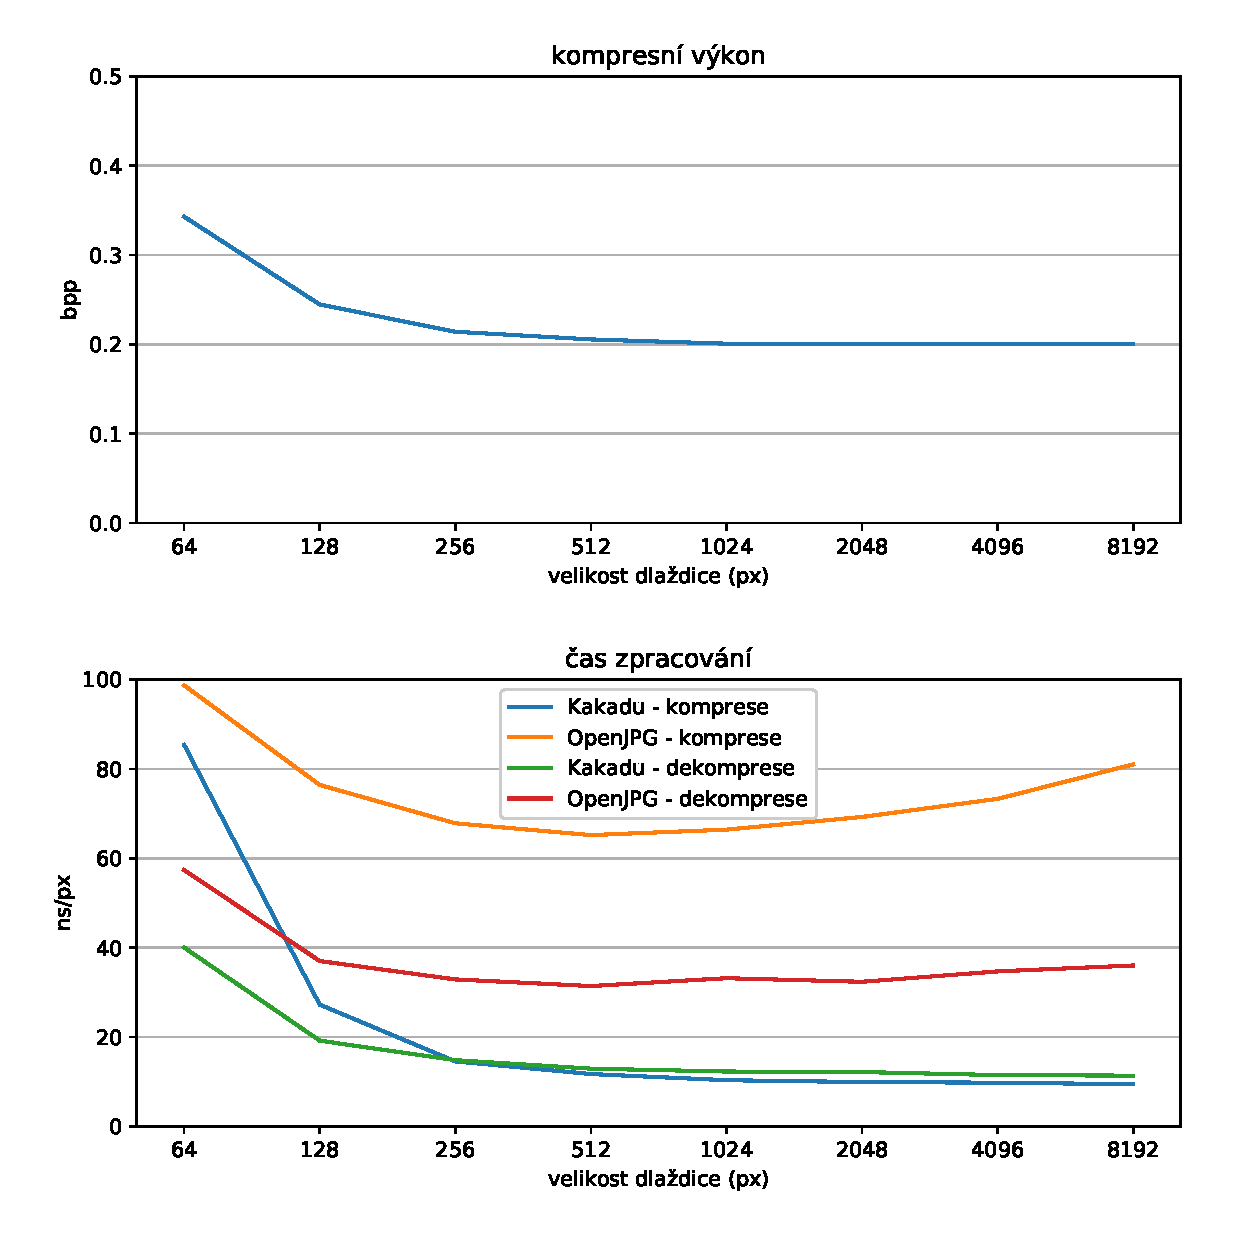
\includegraphics[width=16cm]{obrazky-figures/tiles/fotky_tiles.eps}
  \caption{Velikost dlaždice - ztrátově.}
\end{figure}

\clearpage

U ztrátové komprese se doporučení profilů dělí na dva tábory. Pro \uv{Fotografie} a \uv{Mapy} dlaždice 1024 px a pro \uv{Bitonální} a \uv{Scany} vypnout systém dělení obrazu úplně. Kompresní výkon se ustaluje při 2048 px. Zvětšovat dlaždice za tuto úroveň má z hlediska velikost smysl pouze u obrazových dat, která obsahují alespoň desítky dlaždic při dané velikosti, což klade velké nároky na rozlišení. Datasety jsou navrženy na maximální měřitelnou velikost dlaždice 8192x8192 px. U takto velkých souborů režie dlaždice nehraje měřitelnou roli, proto lze pozorovat naprosto minimální rozdíl velikostí. Průměr rozdílu mezi velikostí dlaždice 2048x2048 px a maximální měřenou velikostí je u ztrátové komprese \textbf{0.27\%}. Při volbě dlaždic o straně menší než 1000 px je ovšem rozdíl velikostí dramatický. Dlaždice o velikosti 64x64 px zvětší datový tok o \textbf{69.33\%} oproti referenční hodnotě. Dvojnásobná velikost dlaždice způsobí změnu velikosti o \textbf{22\%}. Z hlediska velikosti proto vyplývá, že pokud není rozumný důvod pro užití dlaždic je lepší je nepoužívat. 

\begin{figure}[hbt!]
  \centering
  \hspace*{-0.75cm}
  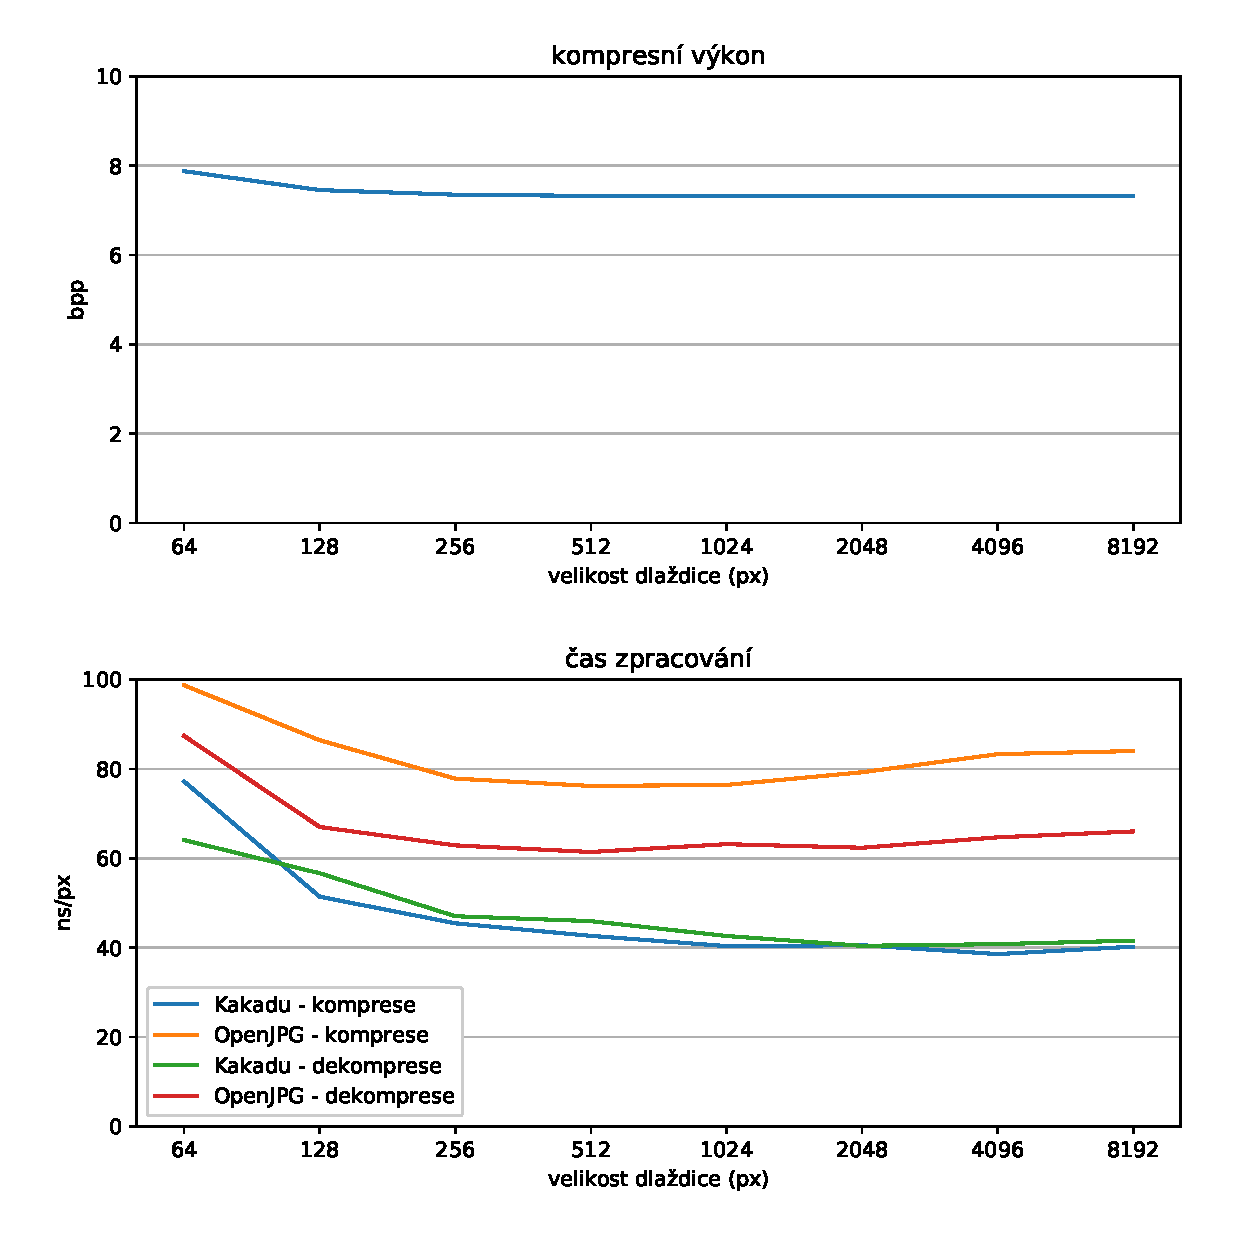
\includegraphics[width=16cm]{obrazky-figures/tiles/fotky_full_tiles.eps}
  \caption{Velikost dlaždice - bezeztrátově.}
\end{figure}

\clearpage
\noindent U bezeztrátové komprese opět doporučují profily dvě nastavení. Pro \uv{Fotografie} a \uv{Bitonální} dlaždice 4096 px a pro \uv{Mapy} a \uv{Scany} vypnout systém dělení obrazu úplně. Závislost kompresního výkonu na dlaždici má zde podobný průběh jako u ztrátové komprese. Rozdíl mezi minimální (64x64 px) a doporučenou (4096x4096 px) je \textbf{9.44\%}. Výpočetní náročnost je také podobná jako u ztrátové komprese. Kakadu se ustaluje pomaleji, OpenJPEG opět za hranicí velikosti dlaždice 1024 px zvyšuje svoji časovou náročnost pro kompresi i dekompresi.

\begin{figure}[hbt!]
  \centering
  \hspace*{-0.75cm}
  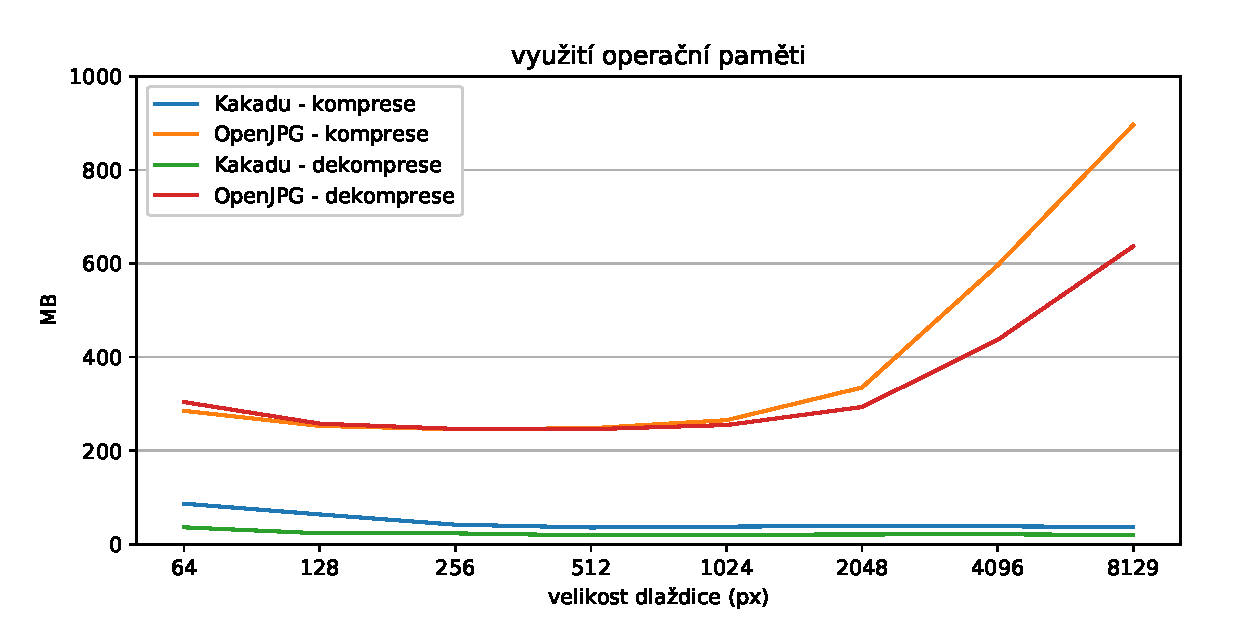
\includegraphics[width=16cm]{obrazky-figures/ram.eps}
  \caption{Vliv velikosti dlaždice na využití operační paměti.}
\end{figure}
\noindent Posledním pomocníkem, který pomůže rozhodnout o velikosti dlaždice je využití operační paměti. Ačkoliv se nejedná o tak uživatelsky postřehnutelný ukazatel jako je kompresní výkon nebo čas zpracování, je nutno jej také brát v potaz.
Obě knihovny u nejmenších dlaždic (64 px a 128 px) využívají určité množství paměti, které přímo nesouvisí s velikostí dlaždice, dle mého odhadu se může jednat o alokaci paměti pro částečné simultánní zpracování. Následně se odehrává pokles. Kakadu se u hranice 512 px srovná a již další paměť nevyžaduje. OpenJPEG opět ukazuje své implantační slabosti. Od hranice 1024 px dramaticky stoupá využití paměti. Je pravděpodobné, že načítá celou dlaždici do paměti, kdežto Kakadu pravděpodobně pracuje se stejně velkými bloky nezávisle - od určité úrovně - na velikosti dlaždice. V extrémních případech OpenJPEG - nezobrazeno v grafu, obsahuje zprůměrovaná data všech datasetů - při kompresi s velikostí dlaždice 8912 px souborů s rozlišení 400 MPx a více při nezkomprimované velikosti 1-2 GB spotřebovával ve špičkách až \textbf{3.8 GB} operační paměti.\\
Kakadu lze doporučit při ztrátové kompresi velikost dlaždice \textbf{1024 px a výše} (zde se spíše odvíjí od velikosti samotného obrazu). Vypnutí systému dělení obrazu poskytuje zanedbatelné zrychlení v časové i velikostní doméně. To samé platí i pro bezeztrátovou kompresi. U OpenJPEG lze vydat konkrétnější doporučení. Z hlediska kompresního výkonu se jeví opět 1024 px a více jako vhodná volba. Časová i paměťová náročnost o obou typů kompresí hovoří jasně v neprospěch zvyšovaní velikosti dlaždice za hranici \textbf{1024 px}. Vypnutí systému dělení u velkých obrazových dat způsobí to stejné, jako velká dlaždice, proto jej nelze u OpenJPEG doporučit pro žádný z datasetů.

% \todo{Graf pameti vyuziti pameti komprese}
% \todo{Graf vyuziti pameti dekomprese}
% \todo{Tabulka}

\clearpage
\newpage
\subsection*{Posun dlaždice a obrazu}
Lze libovolně měnit začátek zpracovávaného obrazu i dat. Vhodné je to například pro zajištění zpracování určitého oblasti v plné velikosti dlaždice. Ty mají jasně definovanou velikost, nicméně ty z kraje obrazu mají takovou velikost, jaká na ně při ořezu vyjde. Postupuje se od levého horního rohu. Tento parametr patří do specifických pro konkrétní obraz, proto byl vyšetřován pouze interně a jeho výsledky - zhoršení kvality při posunu dlaždice v jednotkách procent její velikosti - nelze reprezentativně vztáhnout na celé datasety.

% =======================================================================
% -----------------------------------------------------------------------
%
% ROI
%
% -----------------------------------------------------------------------
% =======================================================================
\subsection*{Regiony zájmu}
Další funkcionalita formátu JPEG 2000, která umožňuje zpracovat určitou část obrazu jinak než ostatní části \cite{roi}. Na rozdíl od dělení dlaždicemi jsou regiony zájmu méně flexibilnější nástrojem. Vznikají až v okamžiku provedení vlnkové transformace. Její koeficienty jsou v regionu zájmu \uv{učiněny důležitějšími} bitovým posunem vlevo, tak aby byly obsaženy ve vyšších bitových rovinách pro dřívější zakódování. Do výsledného souboru jsou poté uložena metadata umožnující zpětný posun koeficientů pro zpětné dekódování. 

\begin{figure}[hbt!]
  \centering
  \hspace*{-0.75cm}
  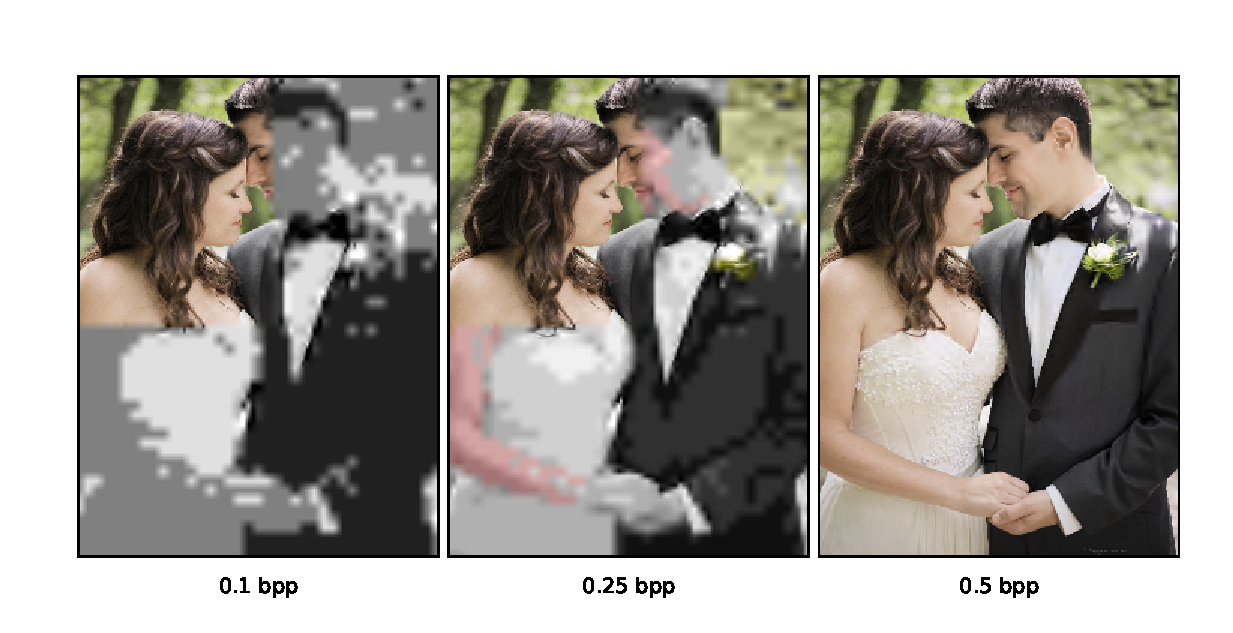
\includegraphics[width=16cm]{obrazky-figures/roi/roi.eps}
  \caption{Regiony zájmu při postupném zvyšování bitové hloubky.}
\end{figure}

% =======================================================================
% -----------------------------------------------------------------------
%
% Wave
%
% -----------------------------------------------------------------------
% =======================================================================
\newpage
\subsection*{Vlnka}
JPEG 2000 používá dvě hlavní vlnky vlnkové transformace. Obě jsou z rodiny biortogonálních spline vlnek. Většina knihoven volbu vlnky vůbec neumožňuje, implicitně používají CDF 5/3 pro bezeztrátovou kompresi a CDF 9/7 pro ztrátovou. Kakadu umožňuje tuto volbu nechat na uživateli. 
% \todo{Bezeztratovou vlnku lze pouzit i pro ztratovou kompresi}
% \todo{Lze vypnout a nastavit}

\begin{figure}[hbt!]
  \centering
  \hspace*{-0.75cm}
  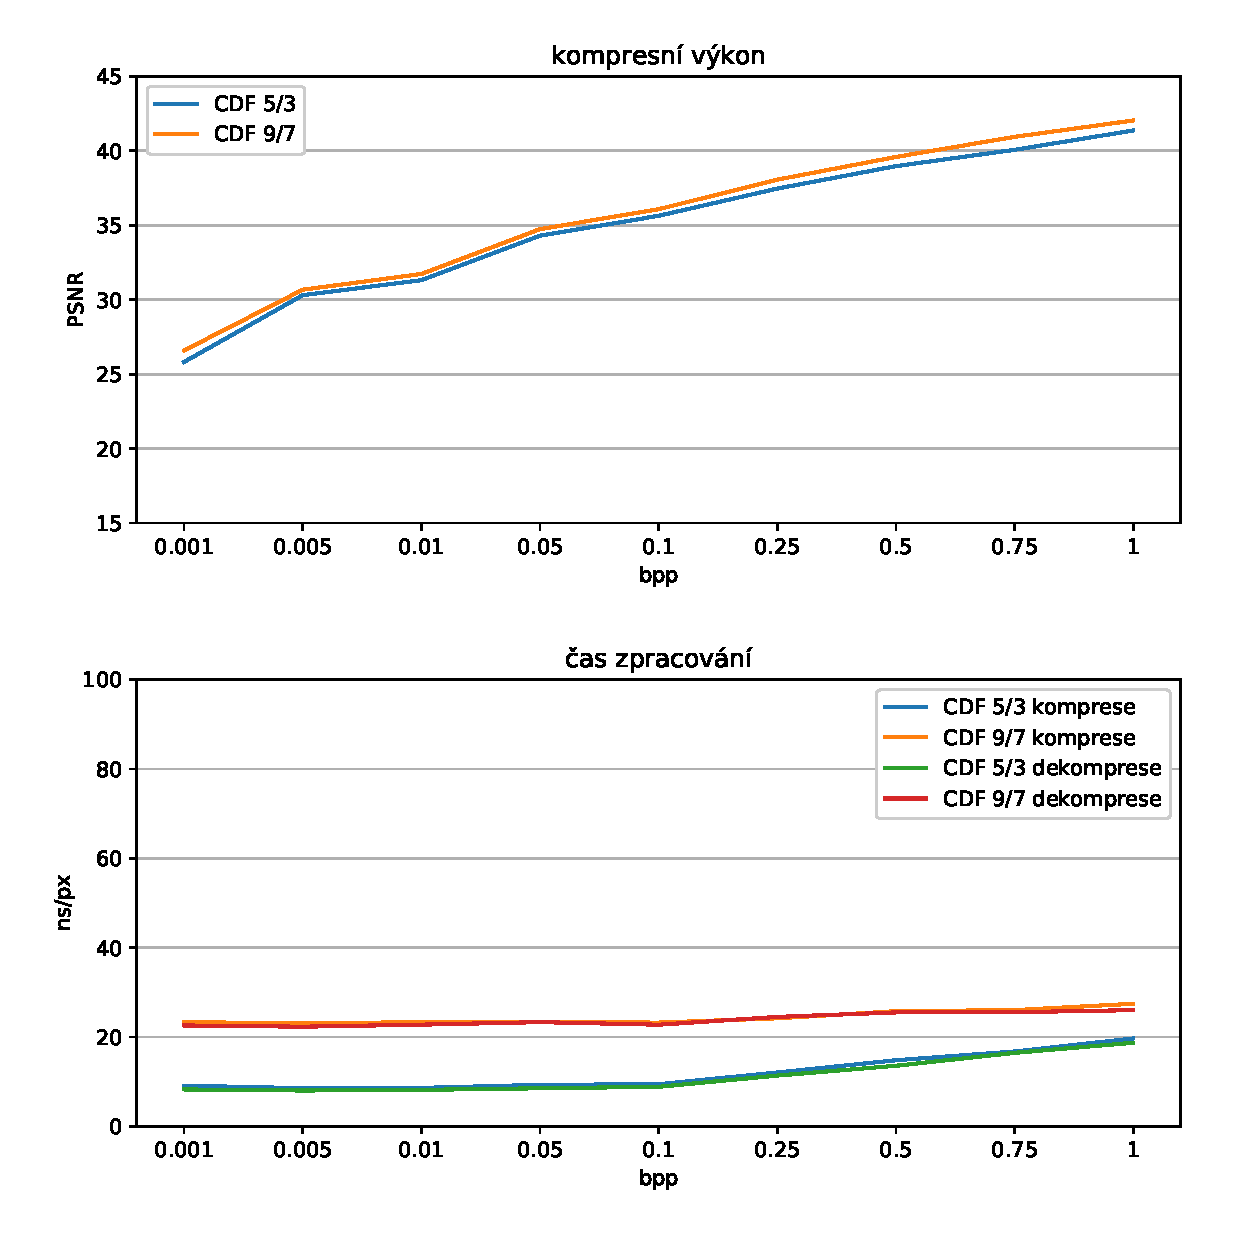
\includegraphics[width=16cm]{obrazky-figures/waves/fotky_waves.eps}
  \caption{Vliv použité vlnky na transformaci při ztrátové kompresi.}
\end{figure}
\noindent Byl vyšetřen kompresní výkon ztrátové komprese vlnek standardně používaných pro oba typy kompresí. Kompresní výkon je očekávatelně lepší u CDF 9/7, která je určená pro tento typ zpracování, a to o \textbf{4.37\%}. Mnohem zajímavější je rozdíl v času komprese a dekomprese. U malých bitových hloubek je CDF 5/3 pro ztrátovou kompresi lepší, ale později se rozdíl smazává.


% % =======================================================================
% % -----------------------------------------------------------------------
% %
% % Quantization step
% %
% % -----------------------------------------------------------------------
% % =======================================================================
% \newpage
% \subsection*{Kvantizační krok}
% Kvantizace koeficientů, který vznikly při vlnkové transformaci je důležitá část procesu komprese.
% % \todo{Rovnice}
% % \todo{Proc se to pouziva}

% \begin{figure}[hbt!]
%   \centering
%   \hspace*{-0.75cm}
%   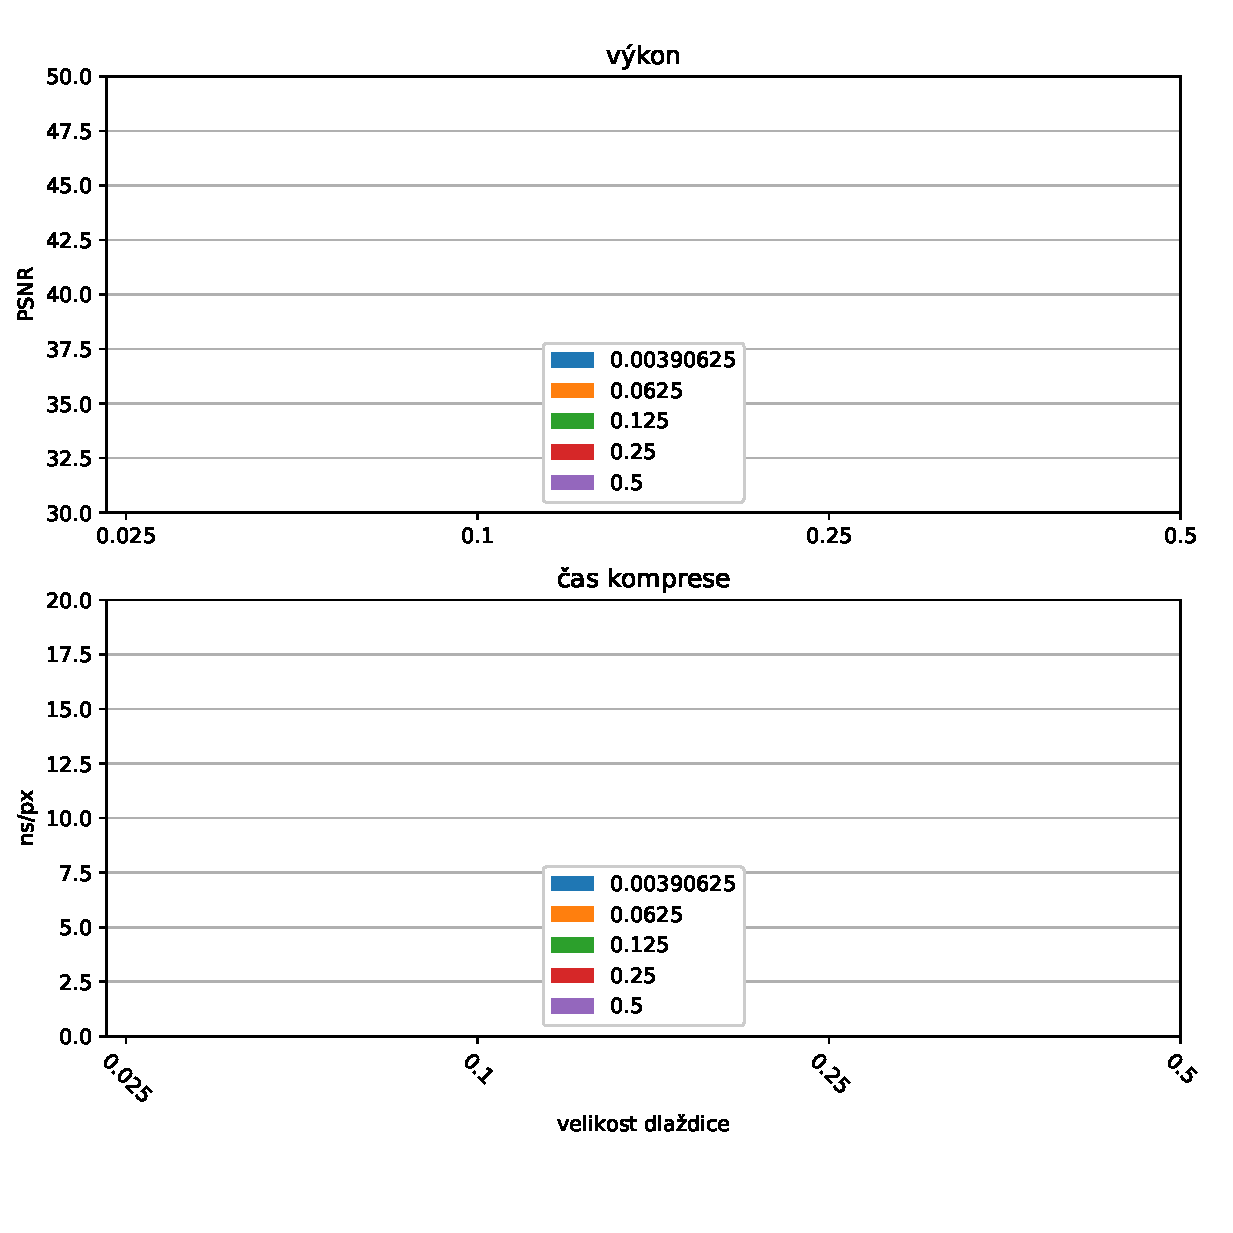
\includegraphics[width=16cm]{obrazky-figures/offset/fotky_offset.eps}
%   \caption{Vyšetřování kvantizačního kroku}
% \end{figure}

% =======================================================================
% -----------------------------------------------------------------------
%
% Levels
%
% -----------------------------------------------------------------------
% =======================================================================
\newpage
\subsection*{Dekompoziční úrovně}
Další z parametrů, který má zásadní vliv na kompresní výkon. Určuje počet provedení dekompozice na podpásma vstupního obrazu. Obor hodnot testování byl zvolen vzhledem k profilů - naprostá většina doporučuje hodnoty 5 až 7 - a smyslu vyšetřování, kdy je maximální počet dekompozičních úrovní určen velikostí obrazu dle druhého násobku počtu úrovní násobeného velikostí code-bloku. Nyní už začíná být jasný výběr doporučené hodnoty. Při šestiúrovňové dekompozici s velikostí code-bloku 64x64 je vyžadováno, aby měl obraz alespoň 4094x4096 px. Rozumné maximum vyšetřování je 8 dekompozičních úrovní. Obě knihovny se v kompresním výkonu shodují, stejně tak jako s průběhem časové náročnosti, s malými výjimkami, které jsou vysvětleny dále. Testování je dle výsledků rozděleno na tři části.

\begin{figure}[hbt!]
  \centering
  \hspace*{-0.75cm}
  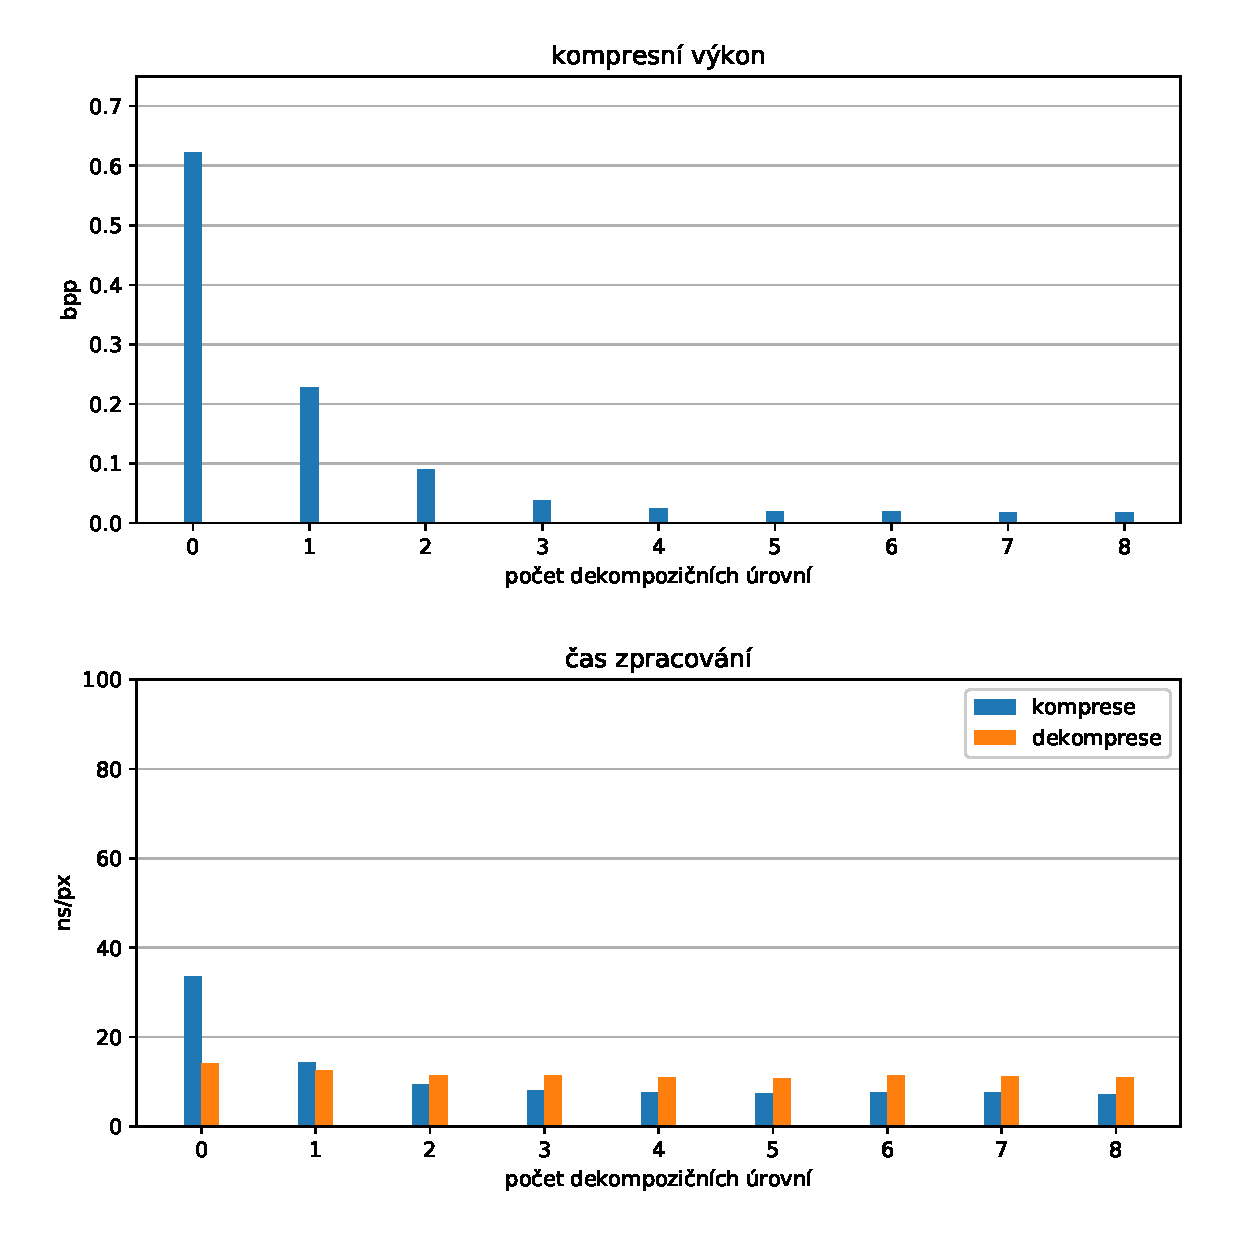
\includegraphics[width=16cm]{obrazky-figures/levels/fotky_levels.eps}
  \caption{Dekompoziční úrovně datasetu \uv{Fotky}.}
\end{figure}

\noindent První části je dataset \uv{Fotografie}. Vlnková transformace je dozajista nutná pro tento typ obrazových dat. Profilem doporučených 5 úrovní zhruba odpovídá naměřeným výsledkům. Nejlepšího kompresního výkonu je dosaženo při 6 úrovních. Po překonání této hranice kompresní výkon mírně klesá, rozdíl mezi 6 a 8 úrovní je \textbf{3.4\%}. Při pohledu do grafu časové náročnosti, lze předchozí verdikt potvrdit. Ačkoliv je graf sjednocen pro obě knihovny, OpenJPEG vykazuje u tohoto datasetu značné zhoršení časové náročnosti pouze při 8 úrovních. Důvodem je pravděpodobně kvalita implementace.

\begin{figure}[hbt!]
  \centering
  \hspace*{-0.75cm}
  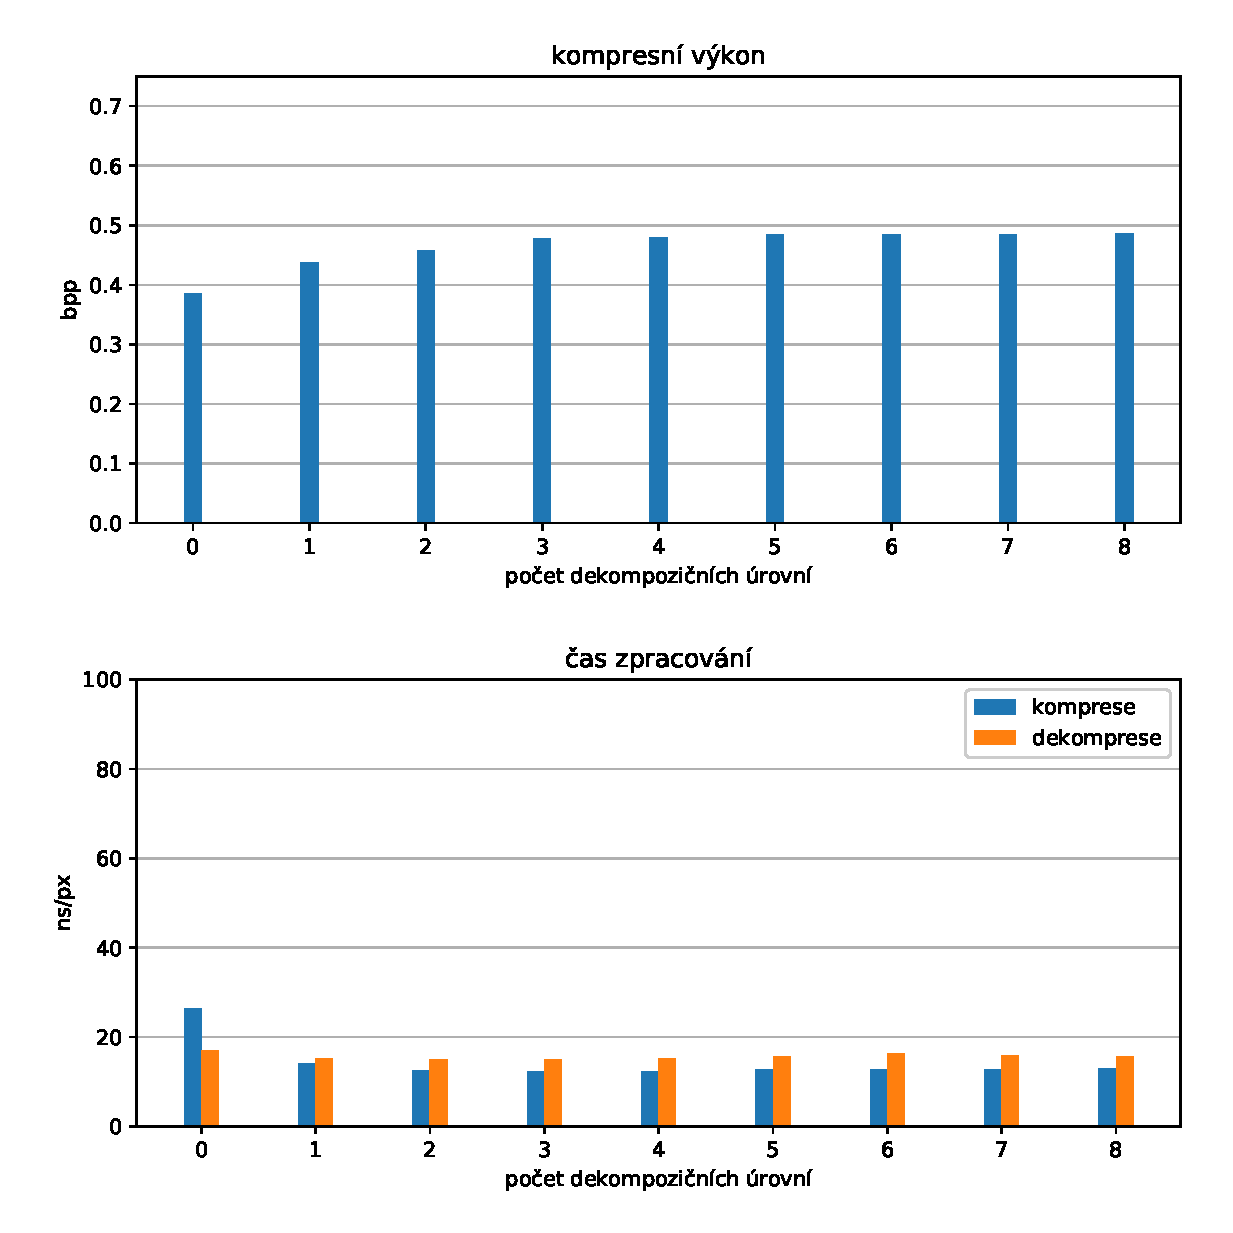
\includegraphics[width=16cm]{obrazky-figures/levels/bitonal_levels.eps}
  \caption{Dekompoziční úrovně datasetů \uv{Bitonální RGB24} a \uv{Bitonální Gray8}.}
\end{figure}

\noindent \uv{Bitonální} obrazová data tvoří další část. Domněnka o relativně malém počtu úrovní se ukázala býti správná, z testů nejlépe vyšla varianta neprovádět dekompozici. Profily se tentokrát příliš netrefily, ale je to logické vzhledem k exotičnosti dat. Po širším vyšetřování byla nalezna pradevědpobná příčina. Při zvolené dekompozici docházelo ke slévání jednotlivých pixelů, kdy na malém prostoru může být ostrá změna jasu i po jednom pixelu. Časová náročnost mluví v neprospěch vynechání dekompozice, ale kompresní výkon je v tomto případě důležitější. Lze doporučit vynechání dekompozice.

\begin{figure}[hbt!]
  \centering
  \hspace*{-0.75cm}
  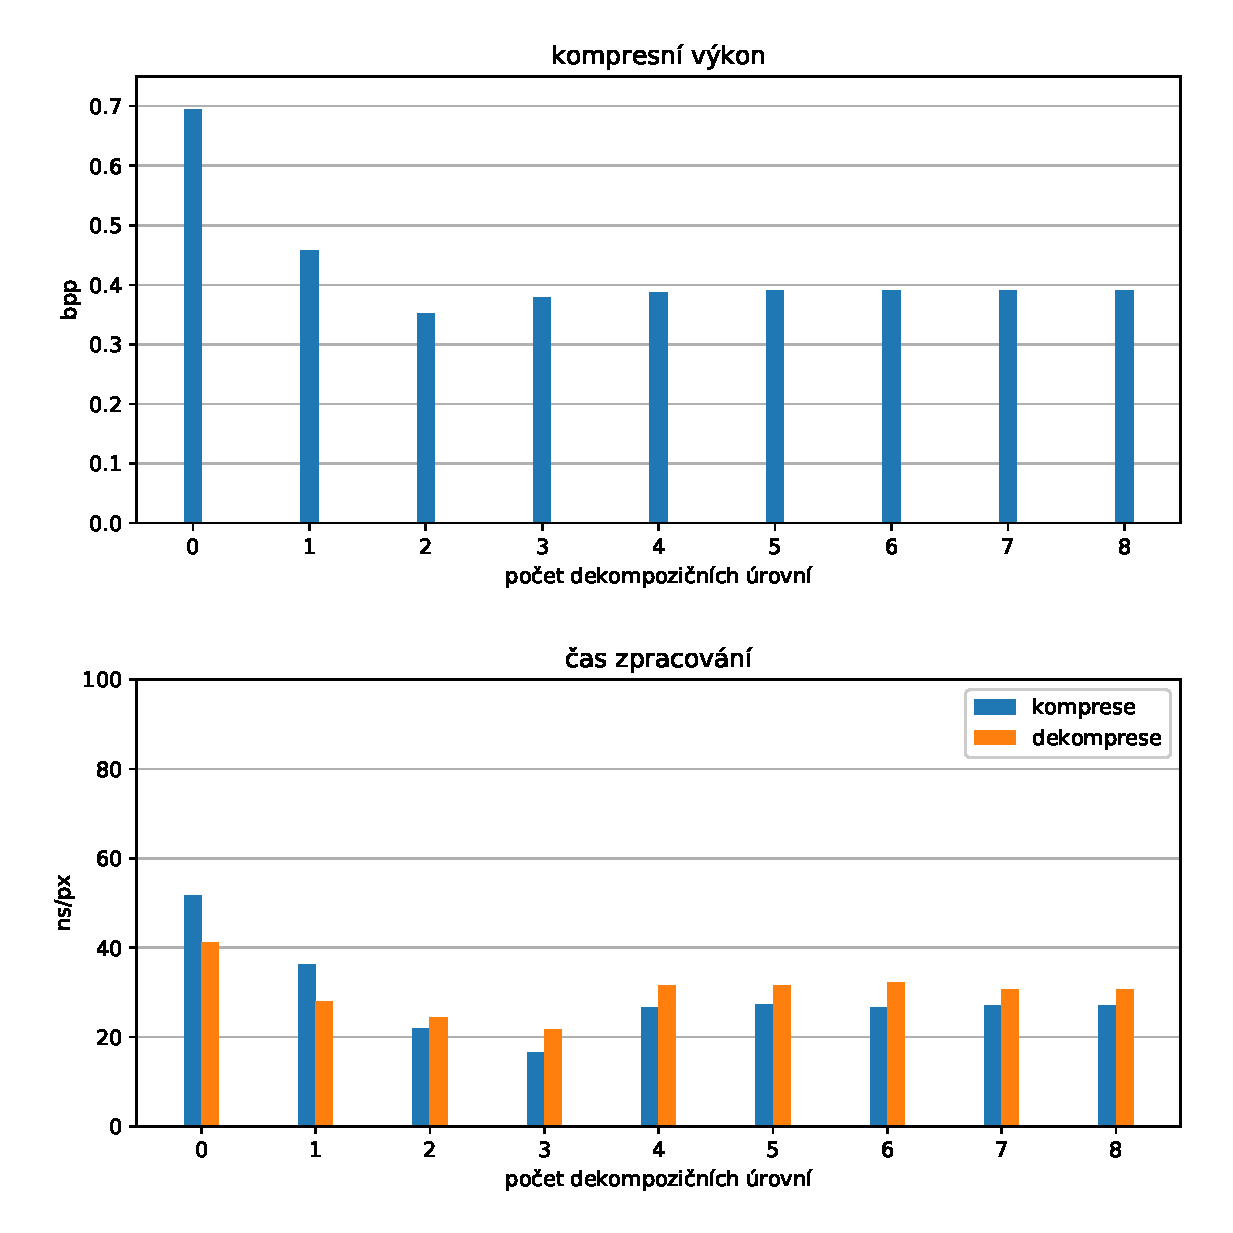
\includegraphics[width=16cm]{obrazky-figures/levels/mapy_levels.eps}
  \caption{Dekompoziční úrovně datasetů \uv{Mapy} a \uv{Scany}}
\end{figure}
\noindent Nakonec jsou vyšetřeny datasety \uv{Mapy} a \uv{Scany}. Profily opět doporučují 5 až 6 úrovní. Skladba dat se oproti datasetu \uv{Fotografie} liší, avšak stále se jedná o třísložkový obrazový materiál s dostatečnou diverzitou obsahu. Počet dekompozičních úrovní o hodnotě 2 se ukázal jako nejlepší. Je pravděpodobné, že tento typ obrazového materiálu sice má dostatečnou diverzitu, avšak je rozložena řídce po obraze. Text nebo rukopis na manuskriptu zabírá malou část obrazu, zbytek je papír, který tvoří relativně homogenní plochy, jejíchž přílišná dekompozice pouze vytváří kompresní artefakty a nepřesnosti. Graf časové náročnosti signalizuje nejlepší výsledky u trojnásobné dekompozice (rozdíl \textbf{18.79\%}, ale stejně jako u předchozího vyšetřování má kompresní výkon přednost.\\
Celkově lze doporučit nejvyšší počet dekompoziční úrovní u datasetu \uv{Fotografie} \textbf{6}, následované \uv{Scany} a \uv{Mapy} s \textbf{2} a \uv{Bitonální} \textbf{nerozkládat}.

\clearpage

% =======================================================================
% -----------------------------------------------------------------------
%
% Code block
%
% -----------------------------------------------------------------------
% =======================================================================
\newpage
\subsection*{Precincty}
Naprostá většina profilů pracující s první částí standardu JPEG 2000 buď nedefinuje jejich použití nebo - při použití alespoň třech dekompozičních úrovní DWT - volí velikosti $256x256$ px pro první úroveň a $128x128$ px pro zbylé. Vliv ztrátové a bezeztrátové komprese nemá smysl vyšetřovat, jedná se pouze o organizaci výstupních dat.

\begin{figure}[hbt!]
  \centering
  \hspace*{-0.75cm}
  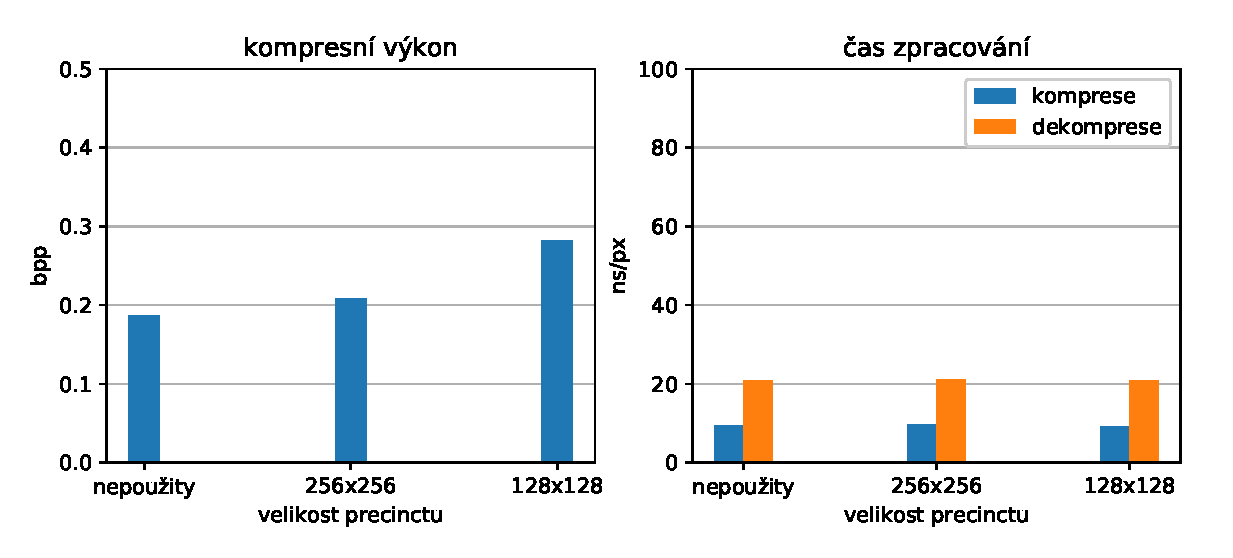
\includegraphics[width=16cm]{obrazky-figures/prec/fotky_prec.eps}
  \caption{Vliv velikosti a použití precinctů.}
\end{figure}

\noindent Čím menší precinct, tím více paketů a tedy větší režie. Velikost 256x256 px zhorší kompresní výkon o \textbf{16.62\%}, u dvojnásobně menších precinctů - a tedy dvojnásobně většího počtu paketů o \textbf{61.02\%}. S počtem paketů roste poměr metadat na úkor užitných dat.
\clearpage

% =======================================================================
% -----------------------------------------------------------------------
%
% Code block
%
% -----------------------------------------------------------------------
% =======================================================================
\subsection*{Code-blok}
Na rozdíl od precinctu se code-blok nemusí striktně držet čtvercových rozměrů, avšak je omezen explicitně daných počtem zpracovávaných hodnot (4096) a velikostí jedné strany (64 px). Drtivá většina dostupných profilu doporučuje maximální velikost 64x64, u bezeztrátové komprese a datasetů profil pro \uv{Mapy} a \uv{Scany} doporučuje použití code-bloku 32x32 px. \\
\begin{figure}[hbt!]
  \centering
  \hspace*{-0.75cm}
  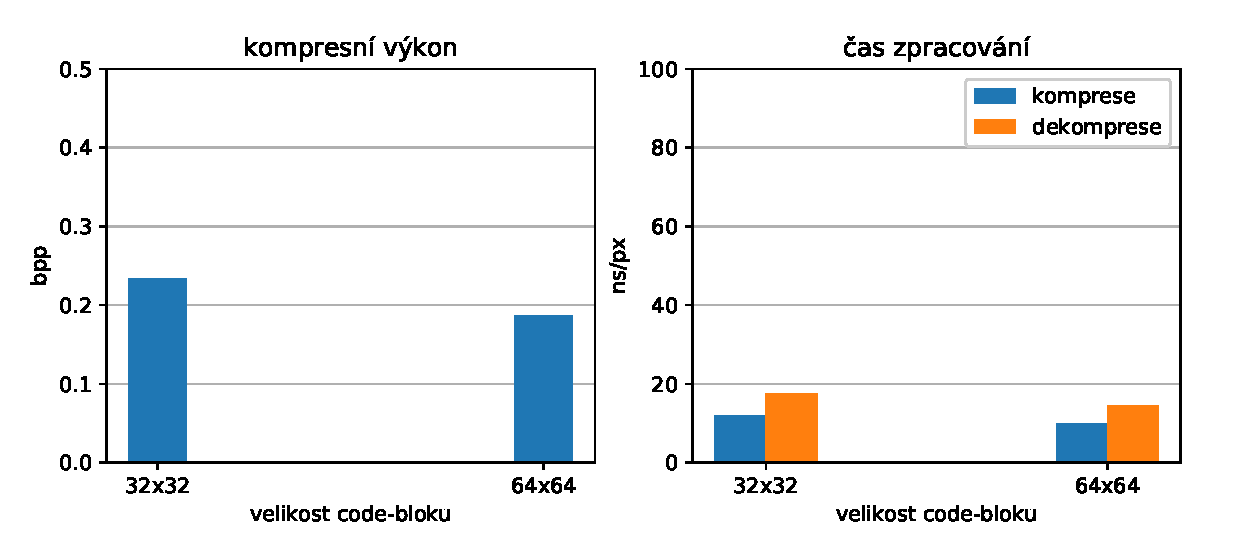
\includegraphics[width=16cm]{obrazky-figures/blocks/fotky_blocks.eps}
  \caption{Vliv velikosti code-blok.}
\end{figure}

\noindent I v tomto případě je verdikt jasný z letmého pohledu do grafu. Při použití code-bloků velikosti 32x32 px se zhorší kompresní výkon o \textbf{27.44\%} a časová náročnost vzroste o \textbf{19.71\%}. Jiné velikosti než 64x64 px mají svůj význam při exotických velikostech precinctů nebo vstupních datech.
\clearpage

% =======================================================================
% -----------------------------------------------------------------------
%
% Order
%
% -----------------------------------------------------------------------
% =======================================================================
\newpage
\subsection*{Pořadí přenosu}
Další z parametrů, který přímo neovlivňuje kompresní výkon, ale určuje organizaci přenosu. Tato vlastnost je velmi žádána např. při přenosu po linkách s omezenou kapacitou. Uživatel je obsloužen vizuálním vjemem, jehož kvalita se zvyšuje s rostoucím počtem obdržených dat. Tento parametr nebude exaktně vyšetřován, ale bude demonstrován jeho dopad v praxi. Definice \uv{kvality} v tomto případě nahrazena čtyřmi měřítky, podle níž je kvalita škálována. První z nich je vrstva (\textit{quality}). Pokud je přenášený obraz komprimován s vrstvami, jsou s postupným nárůstem přenesených dat protkávány a tím se zvyšuje kvalita. Další je rozlišení (\textit{resolution}). Nejedná se o rozlišení ve smyslu dekompozičních vrstev, ale o rozlišení obrazu. Na začátek souboru je zakódován malý náhled. Rozlišení roste v násobcích dvou. Škálovat lze také pomocí pozice (\textit{spatial location}). Pozicí jsou myšleny části obrazu, které se přenášejí za sebou shora dolů, vhodné například pro tiskárny a paměťově omezené aplikace. Poslední je komponenta (\textit{component}) což jsou u vyšetřovaných datasetů složky barevného prostoru. Tento parametr je zadáván jako čtyř znaková kombinace. Např. LRCP, první písmeno znamená složku, která bude postupovat nejpomaleji a poslední nejrychleji. 

\begin{figure}[hbt!]
  \centering
  \hspace*{-0.75cm}
  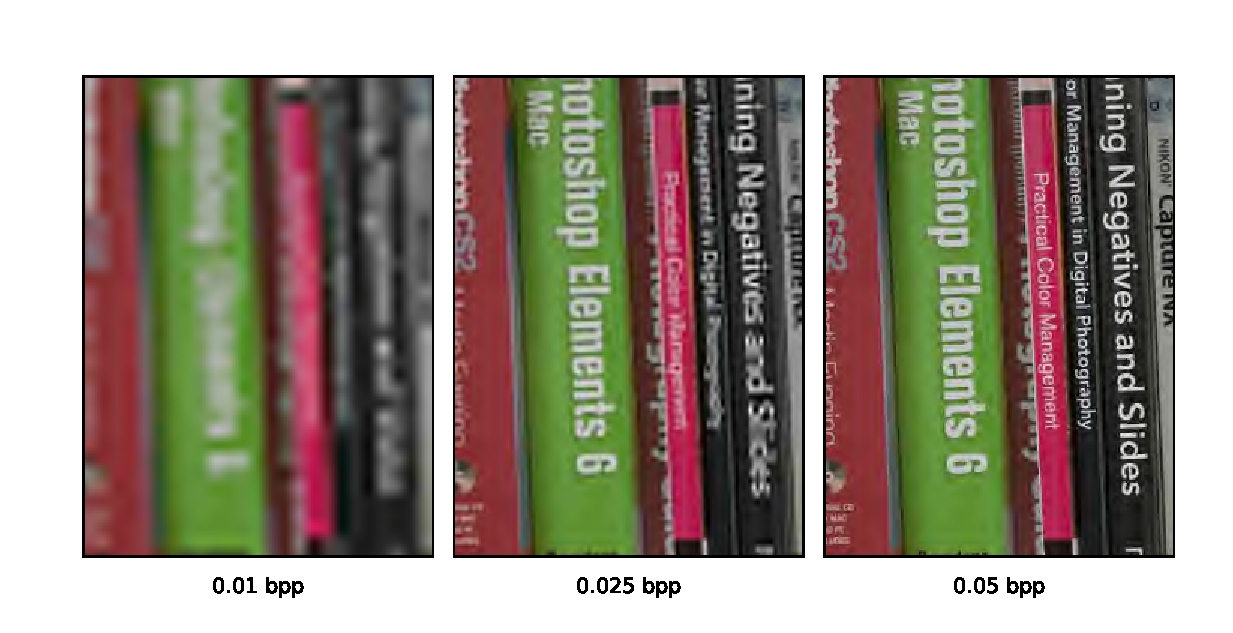
\includegraphics[width=16cm]{obrazky-figures/order/lrcp.eps}
  \caption{Pořadí přenosu \textit{LRCP}.}
\end{figure}

U obou knihoven výchozí hodnota nastavení pro tento parametr. Nejrychleji roste pozice následována komponentou, rozlišením a vrstvou. Parametr zde vykazuje nejlepší výsledky. Celkem existuje pět voleb. Níže jsou rozebrány dvě nejčastější v profilech datasetů.
\clearpage
\begin{figure}[hbt!]
  \centering
  \hspace*{-0.75cm}
  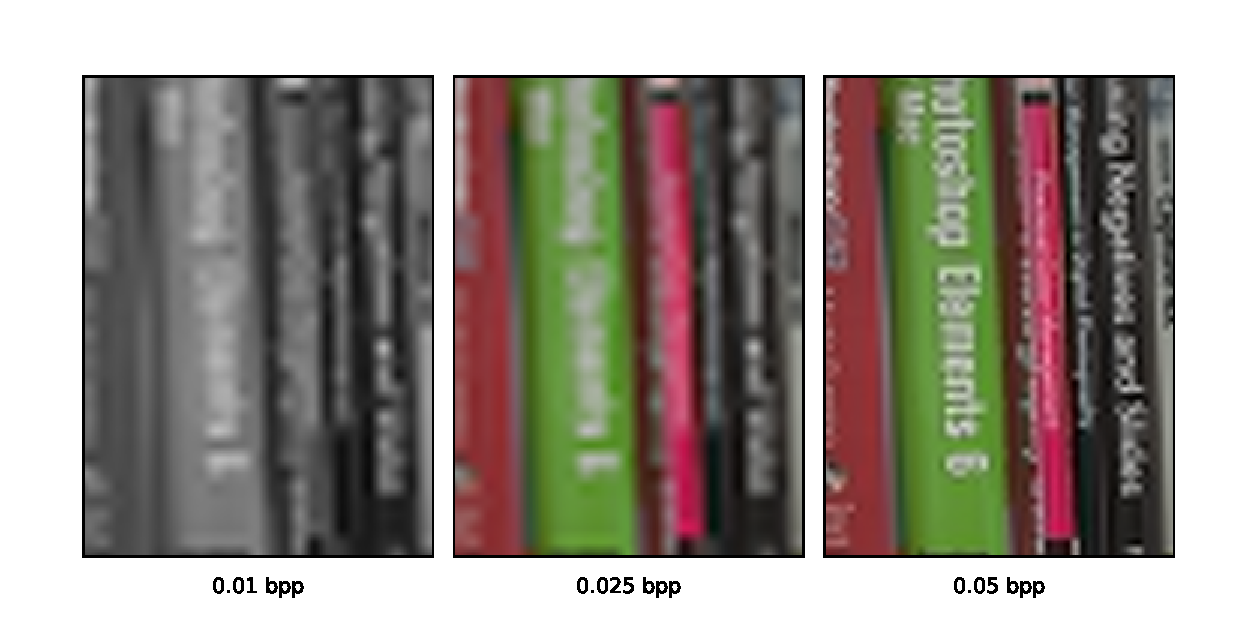
\includegraphics[width=16cm]{obrazky-figures/order/rpcl.eps}
  \caption{Pořadí přenosu \textit{RPCL}.}
\end{figure}

\begin{figure}[hbt!]
  \centering
  \hspace*{-0.75cm}
  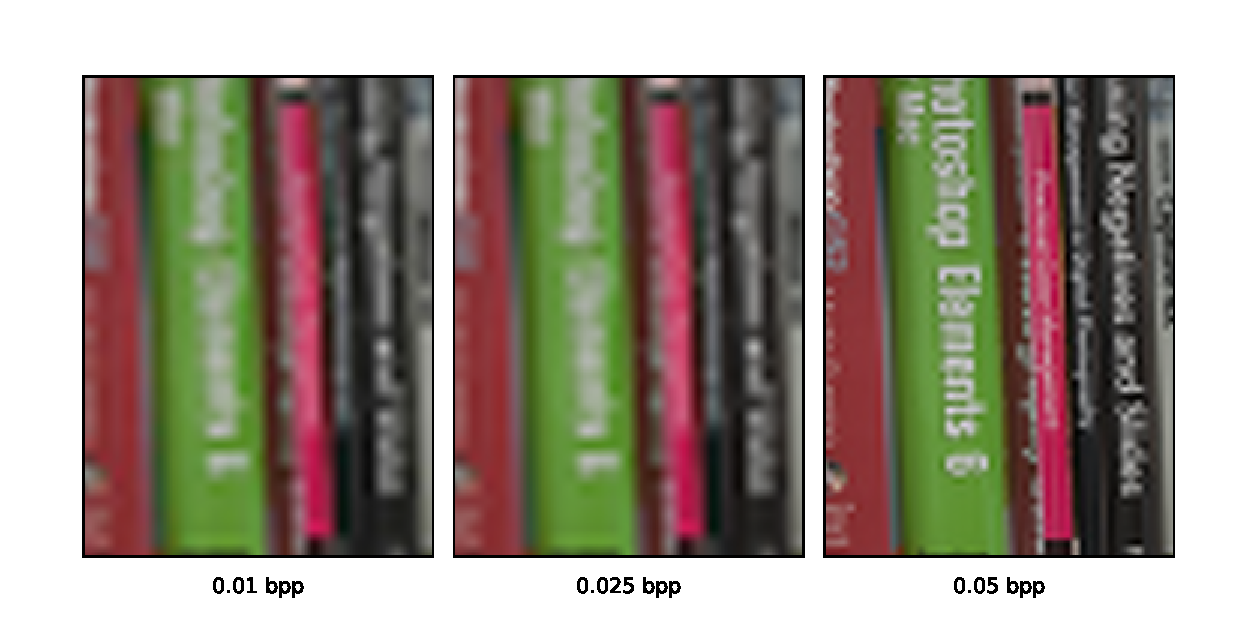
\includegraphics[width=16cm]{obrazky-figures/order/rlcp.eps}
  \caption{Pořadí přenosu \textit{RLCP}.}
\end{figure}

\noindent Striktně dle výsledku vyšetřování komprese lze doporučit pořadí přenosu \textbf{LRCP}. Pořadí neovlivňuje kompresní výkon ani dobu nutnou pro kompresi, proto je toto doporučení volnější a záleží spíše na uživateli, jak hodlá zkomprimovaný soubor používat.  Pouze dataset \uv{Bitonální Gray8} logicky vykazuje lepší výsledky při použití přenosu \textbf{CPRL}, jelikož komponenta je zde jenom jedna.

% \begin{figure}[hbt!]
%   \centering
%   \hspace*{-2.5cm}
%   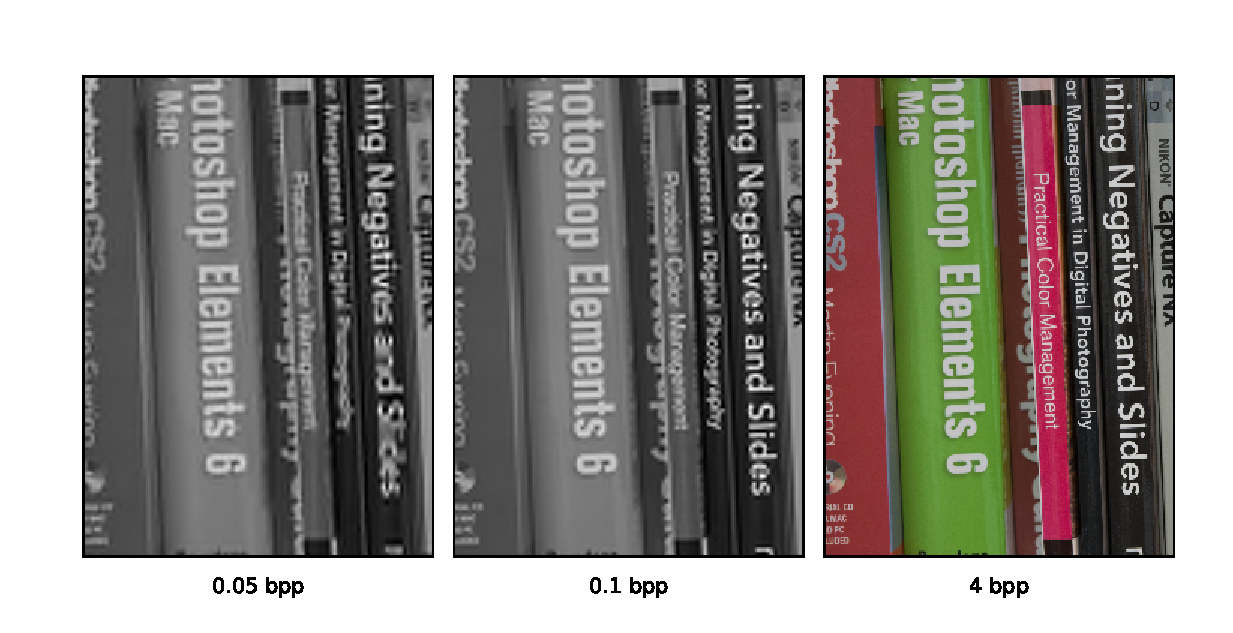
\includegraphics[width=19cm]{obrazky-figures/order/cprl.eps}
%   \caption{Vyšetřování průběhů kvality komprese datasetu \textit{Scany}}
% \end{figure}
\clearpage

% \begin{figure}[hbt!]
%   \centering
%   \hspace*{-2.5cm}
%   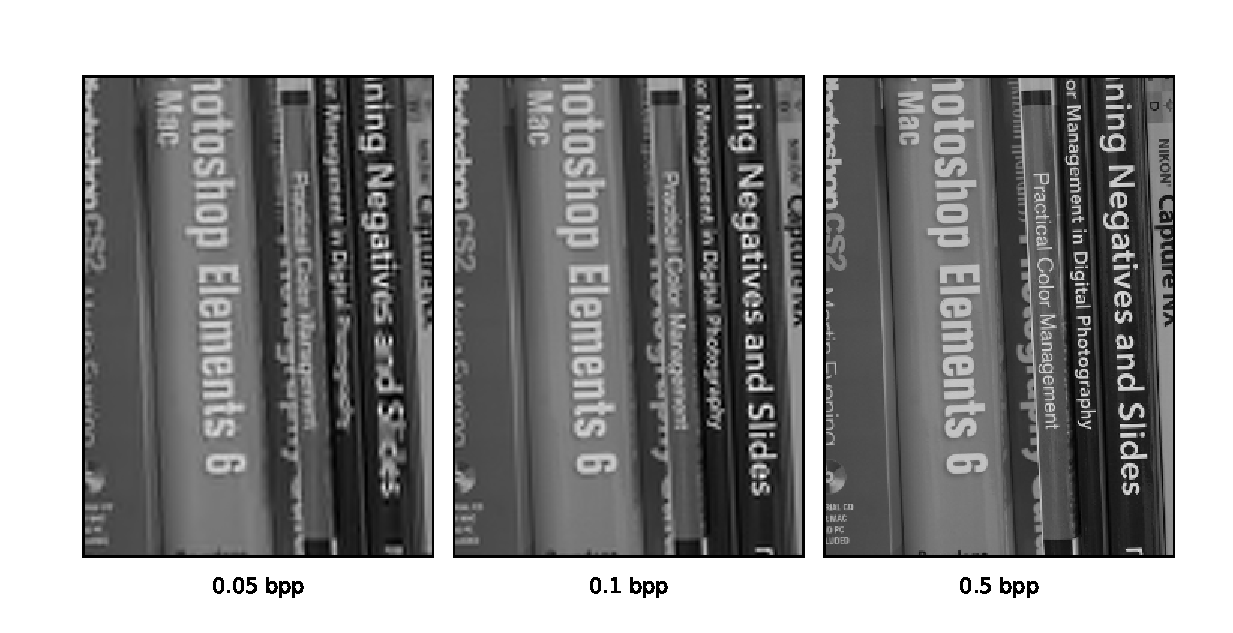
\includegraphics[width=19cm]{obrazky-figures/order/pclr.eps}
%   \caption{Vyšetřování průběhů kvality komprese datasetu \textit{Scany}}
% \end{figure}



% =======================================================================
% -----------------------------------------------------------------------
%
% Vrstvy kvality
%
% -----------------------------------------------------------------------
% =======================================================================
\newpage
\subsection*{Vrstvy kvality}
Slouží k uložení více kvalit obrazu do jednoho souboru. Jednotlivé bitové roviny code-bloků jsou v kódovacích průchodech EBCOT prokládány pro určité kvality. Problém toho přístupu je opět - jako u precinctů - režie. Každý code-blok pro každou vrstvu kvality musí být jasně oddělen. V praxi se používají tři přístupy pro použití vrstev. První možnost je použít jenom jednu, což je případ profilů pro bezeztrátovou kompresi. Takto zpracované soubory většinou slouží jako archivní zdroje nebo zálohové soubory, ze kterých jsou tvořeny ztrátové kopie. U nich se využití vrstev vyplatí, stejně tak jako doporučují profily. Pokud jsou známy případy použití, lze ušít přímo na míru kvalitu vrstev (vyjmenovat konkrétní kvality). Tento přístup je nejefektivnější. Poslední přístup je explicitně zadaný počet vrstev s logaritmickým rozložením, čímž je zajištěna škálovatelnost obrazu bez nutné znalosti přesných kvalit.

\begin{figure}[hbt!]
  \centering
  \hspace*{-0.75cm}
  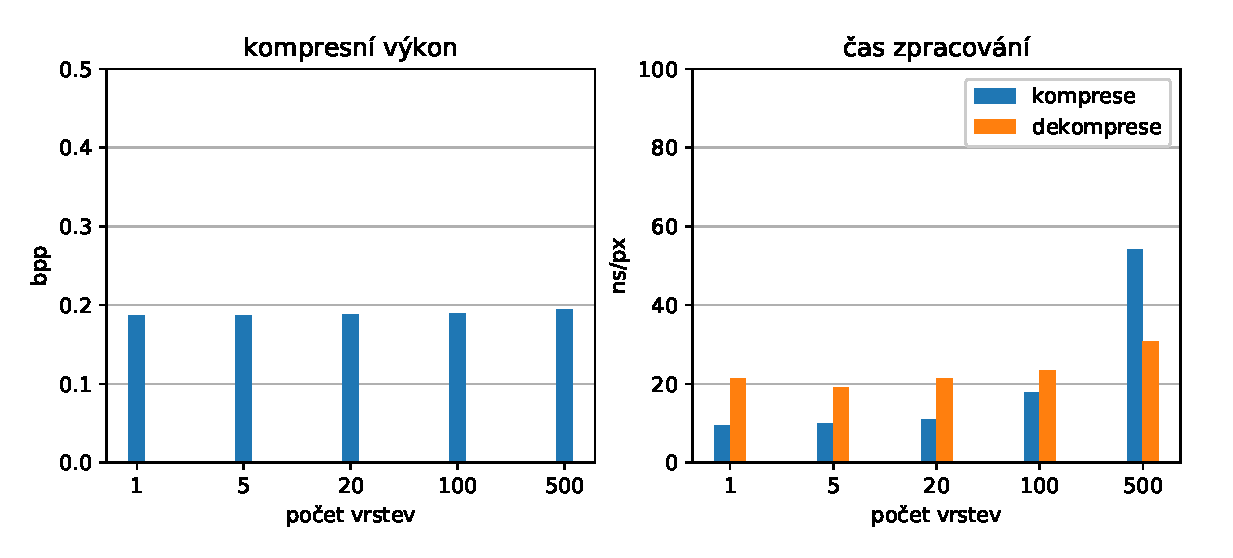
\includegraphics[width=16cm]{obrazky-figures/layers/fotky_layers.eps}
  \caption{Vliv počtu vrstev na kompresní výkon a čas.}
\end{figure}

\noindent Paměťová režie se neukázala při code-bloku 64x64 px jako velký problém, i při stovkách vrstev kvality je nárůst do \textbf{5\%}. Na co naopak počet vrstev má značný vliv je doba komprese. 20 vrstev představuje nárůst od času nutného ke kompresi o \textbf{23.44\%}, 100 vrstev více než dvojnásobek a 500 vrstev sedminásobek. Z výkonnostního hlediska lze doporučit maximálně \textbf{20 až 30} vrstev bez velké výpočetní režie. 
\clearpage

\begin{figure}[hbt!]
  \centering
  \hspace*{-0.75cm}
  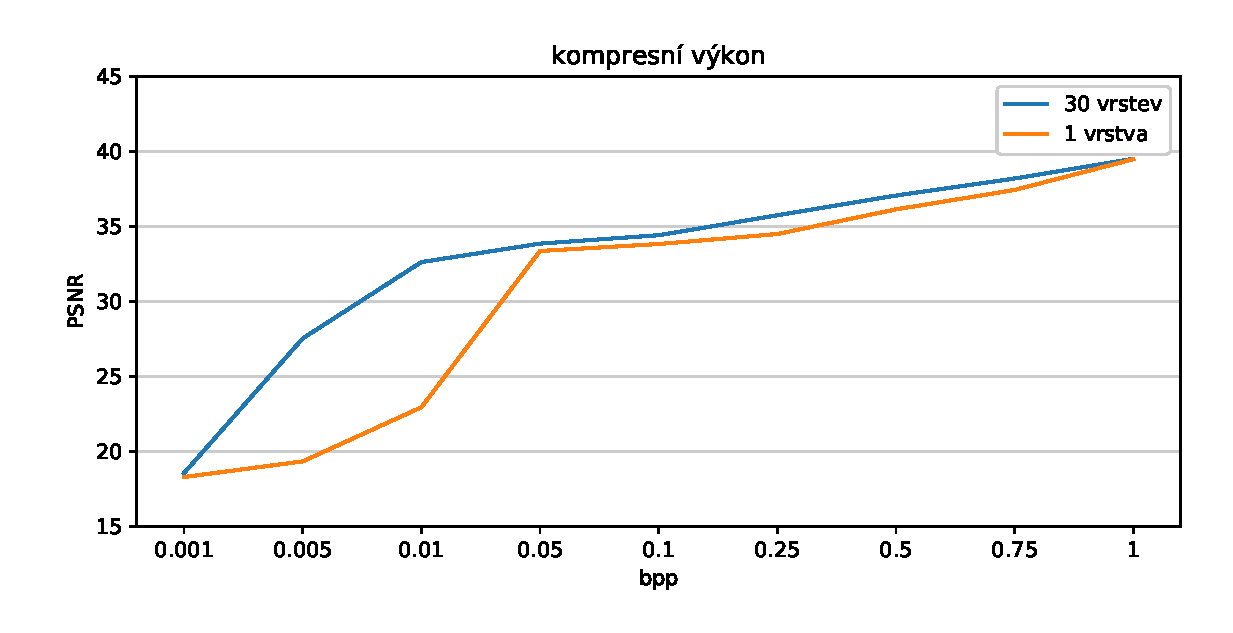
\includegraphics[width=16cm]{obrazky-figures/layers.eps}
  \caption{Průběh kvality pořadím přenosu LRCP s vrstvami a bez.}
\end{figure}
Z předchozího vyšetřování vyplynulo, o kolik při zvolené kvalitě dokáží nafouknout datový tok metadata. Tentokrát je vyšetřena kvalita na intervalu hodnot. Bylo použito 30 vrstev s logaritmický rozsahem v intervalu <0.001, 1>. Pro jednovrstvou kompresi bylo zvoleno 1 bpp. U malých bitových hloubek je rozdíl velmi znatelný, průměrně více než \textbf{85.23\%}. S rostoucí bitovou hloubkou se rozdíl smazává. Profily pro ztrátovou kompresi používají maximálně 7 vrstev, kdy 5 vrstev tvoří kvalitní minimum pro škálovatelné vrstvy. Při použití vrstev lze doporučit hodnotu \textbf{5 až 10} pro běžné případy.

\clearpage

% =======================================================================
% -----------------------------------------------------------------------
%
% Odolnost vůči chybám
%
% -----------------------------------------------------------------------
% =======================================================================
\newpage
\subsection*{Odolnost vůči chybám}
Jako jakýkoliv jiný datový tok, jenž je přenášen po nespolehlivém přenosovém médiu - což je naprostá většina používaných koncovými zákazníky - je jej nutno zabezpečit proti chybám. JPEG 2000 nabízí v dalších částech standardu široké možnosti zabezpečení, nicméně cílem této není práce zevrubně zkoumat zabezpečení, proto jsou vyšetřeny jenom základní parametry. Nejjednodušším způsobem zabezpečení je označit paket. JPEG 2000 pro tuto činnost nabízí dva markery: SOP a EPH. První z nich znační začátek paketu (v datovém toku hodnota větší než FF8F H, což je maximální hodnota dvou datových bitů) a druhý konec. Dále lze instruovat EBCOT tak, aby používal módy určené pro zabezpečení. SEGMARK označní každou bitovou rovinu čtyřbitovou kombinací a ERTERM vynutí standardem definované ukončování bloků zpracovávaných MQ kodérem. Výpočetní náročnost v tom případě nehraje roli, markery pouze zvětší velikost výsledného souboru a zvoleném dva módy EBCOT slouží pouze k označení významných míst v datovém toku.

\begin{figure}[hbt!]
  \centering
  \hspace*{-0.75cm}
  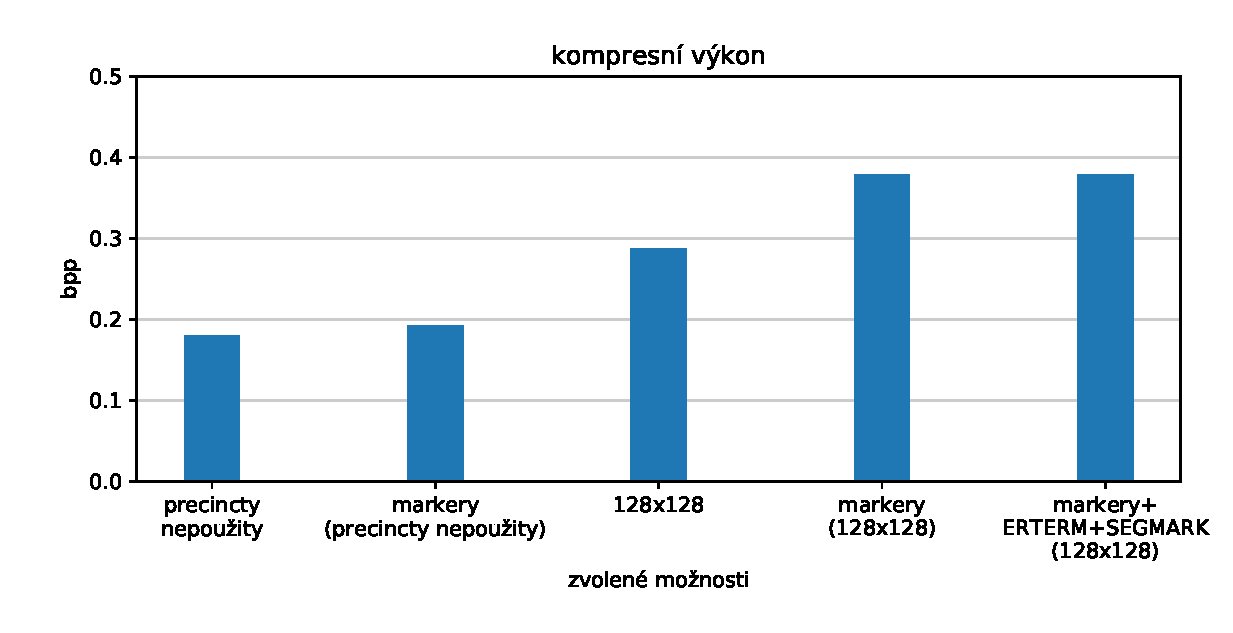
\includegraphics[width=16cm]{obrazky-figures/demand/test.eps}
  \caption{Vliv mechanismů zabezpečení na velikost souboru.}
\end{figure}

\noindent Nejprve byl zakódován soubor bez jakékoliv uživatelem vynutitelné ochrany proti chybám s rozdílnou velikostí precinctu ovlivňující generování paketů. Při označení paketů vzrostla velikost souboru o \textbf{6.48\%}, respektive \textbf{17.41\%} u velikosti precinctu 128x128 px. Použití módů EBCOT nepřineslo měřitelný rozdíl. Profily zabezpečení nedefinují, proto lze doporučit užití módu ERTERM/SEGMARK u obou typů komprese. S markery je nutno být opatrnější. Zhorší kompresní výkon (u malých precinctů značně), proto je jejich užití doporučeno pouze v případě oprávněné obavy o chybný přenos. 
\clearpage

% =======================================================================
% -----------------------------------------------------------------------
%
% Redukce výpočetních nároků
%
% -----------------------------------------------------------------------
% =======================================================================
\newpage
\subsection*{Redukce výpočetních nároků}
Poslední částí testování je zjištování vlivu módů EBCOT na rychlost komprese a dekomprese. Prvním je BYPASS. Ten pracuje na principu přemostění MQ kodéru. Mělo by dojít ke snížení výpočetních nároků bez velké ztráty kvality. Další vyšetřované módy jsou RESET (vyčistí kontextové stavy po každém průchodu) a RESTART (celý kodér je restartován).

\begin{figure}[hbt!]
  \centering
  \hspace*{-0.75cm}
  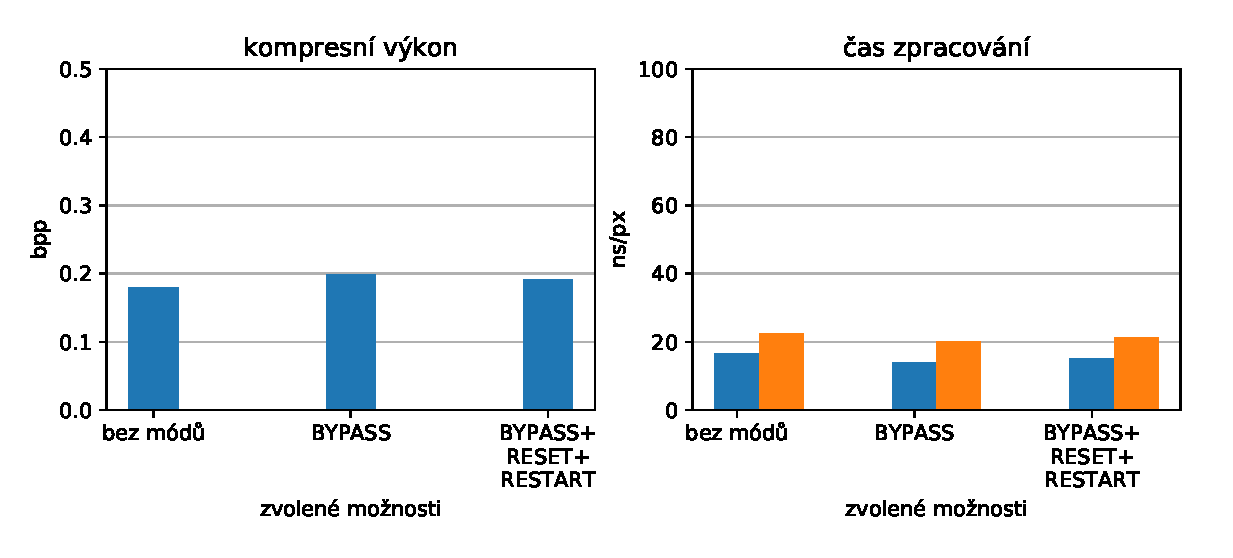
\includegraphics[width=16cm]{obrazky-figures/compute/test.eps}
  \caption{Vliv mechanismů redukce výpočetních nároků na kompresní řetězec.}
\end{figure}

Pro oba typy komprese a všechny datasety došlo ke zhoršení kompresního výkonu o \textbf{7.84\%} pro mód BYPASS a \textbf{5.42\%} pro módy BYPASS, RESET a RESTART. Redukce výpočetních nároků proběhla, avšak ne tak znatelně, o \textbf{8.95\%} pro mód BYPASS a \textbf{3.82\%} pro módy BYPASS, RESET a RESTART.

\begin{figure}[hbt!]
  \centering
  \hspace*{-0.75cm}
  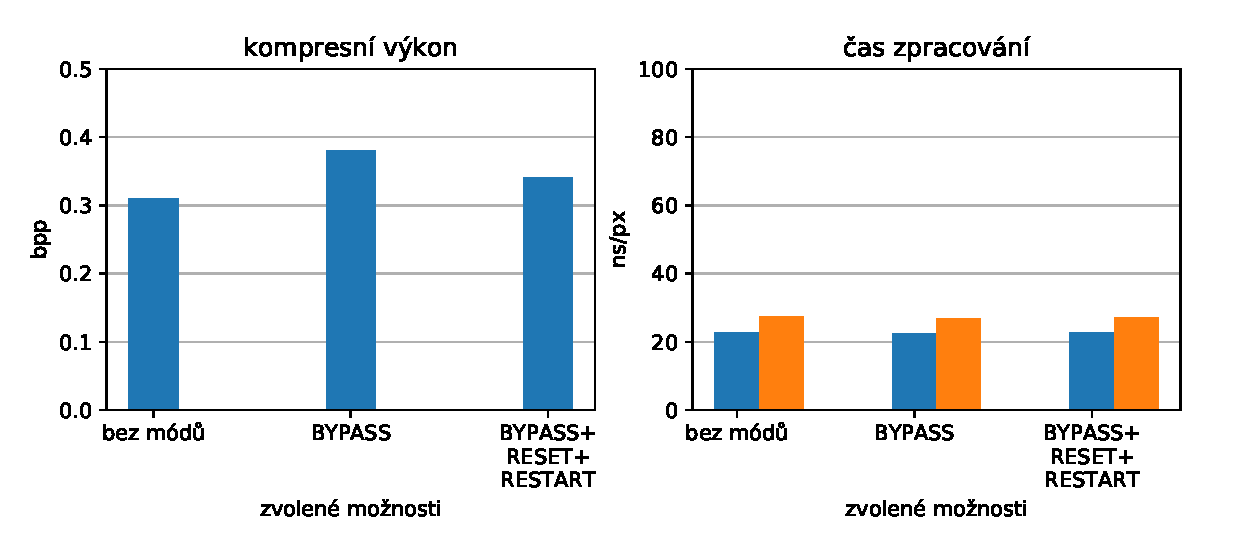
\includegraphics[width=16cm]{obrazky-figures/compute/test2.eps}
  \caption{Vliv mechanismů redukce výpočetních nároků na kompresní řetězec \uv{Bitonální}.}
\end{figure}

\noindent Po bližším zkoumání bylo odhaleno, že oba datasety \uv{Bitonální} vykazují známky výrazného zhoršení kompresního výkonu, konkrétně o \textbf{22.34\%} při velmi malém zlepšení výpočetních nároků \textbf{0.88\%}. Tento fenomén je pravděpodobně způsoben specifickým obsahem zmíněného datasetu. Celkově lze mód BYPASS doporučit pro oba typy kompresí a všechy datasety kromě \uv{Bitonální}. Výhody (rychlost zpracování) převažují nevýhody (zhoršený kompresní výkon). Použití další dvou módů (RESET, RESTART) je více diskutabilní. Mírně zlepší kompresní výkon, avšak výpočetním nárokům pomůžou minimálně. 
% =======================================================================
% -----------------------------------------------------------------------
%
% Doporučené hodnoty
%
% -----------------------------------------------------------------------
% =======================================================================
\newpage
\section{Shrnutí testování}
Byly vyšetřeny parametry pro ztrátovou i bezeztrátovou kompresi pomocí knihoven Kkadu a OpenJPEG. Většina vyšetřování měla za cíl určit vhodnou hodnotu, či obor hodnot, která je v vzhledem ke kompresnímu výkonu, časové a paměťové náročnosti nejlepší. U některých typů vyšetřování ovšem toto postrádalo smysl, a proto byla zvolena forma demonstrace funkcionality (např. ROI, nastavení kompresní vlnky). Nejprve byl vyšetřen rozdíl mezi formáty JPEG a JPEG 2000, kdy druhý jmenovaný jasně ukázal svoji technickou vyspělost, hlavně při velkých kompresních poměrech. Poté následovalo testování parametrů. Převod barevného prostoru ze vstupního RGB do YCrCb se ukázal jako nutný pro oba druhy komprese a všechny datasety, kromě \uv{Bitonální Gray8}, kde kvůli počtu barevných komponent nebylo potřeba tento parametr vyšetřovat. Co ovšem měl smysl vyšetřovat u všech datasetů byla velikost dlaždice. Zde se jasně ukázaly nectnosti implementace OpenJPEG z oblasti časové a paměťové domény, které jasně definovaly, jakou volbu parametru použít. Kakadu naopak využívalo paměť i čas očekávaně. Posun dlaždice a obrazu se neukázaly jako vhodné k zevrubnému vyšetřování. U regionů zájmu byla demonstrována pouze jejich funkčnost, jelikož záleží na konkrétním vstupním obrazu, jak ovlivní kompresní výkon a časovou/paměťovou náročnost. Další z teoreticky vyšetřených parametrů byl typ vlnky při ztrátové kompresi. Tento test mohl být proveden pouze v Kakadu, jelikož OpenJPEG tuto volbu neumožňuje. Vlnka pro bezeztrátovou kompresi dosahovala horších kompresních výkonů, ale menší časové náročnosti. Dekompoziční úrovně opět ukázaly rozdíly mezi datasety, kde \uv{Fotografie} vykazovaly nejlepší výsledky při použití šestinásobného rozkladu, ale \uv{Bitonální} naopak nevyžadují vůbec žádný rozklad. Následovala dvojice precincty a code-bloky, kde byly výsledky očekávatelné, ale nebylo na škodu ukázat, proč se dané hodnoty používají. Pořadí přenosu bylo opět spíše teoretické vyšetřování, kdy z části záleží na volbě uživatele a případu použití dat. Co lze ovšem skoro paušálně doporučit jsou vrstvy kvality. Režie je při jednotkách až desítkách vrstev únosná, pouze při bezeztrátové kompresi archivních originálů má smysl tento mechanismus vypnout. Zlepšení kompresního výkon při použití vrstev je velmi znatelné při postupné dekompresi velkých kompresních poměrů. Nakonec by vyšetřen EBCOT, a to ve dvou testech. První se zabýval zabezpečením. Zde se ukázalo, že použití módů pro zabezpečení je velmi levné z hlediska kompresního výkonu. To samé se ale nedá říci o markerech pro označení paketu. Ty přinášejí značnou režii, kterou je nutno akceptovat pro zabezpečení dat. Druhý se zabýval redukcí výpočetních nároků. Mód BYPASS ukázal svoji sílu při zmenšení časové náročnosti na úkor zhoršení kompresního výkonu. U datasetu \uv{Bitonální} produkoval velmi špatné výsledky, proto jej nelze doporučit plošně. Během testu byly vyšetřeny další módy pro redukci výpočetních nároků (RESTART a RESET). Kakadu bylo při testování průměrně \textbf{2.4x} rychlejší než OpenJPEG. Paměťové nároky byly u Kakadu zhruba \textbf{poloviční}, pouze v extrémních případech - dlaždice - rostly exponenciálně. Některé parametry nešlo vyšetřit za využití obou typů knihoven z důvodu neúplného pokrytí standardu. 

\chapter{Závěr}
\label{zaver}
Práce je složena ze tří částí. V kapitole nazvané \textit{JPEG 2000} proběhlo seznámení se s formátem, kdy jeho předchůdce JPEG posloužil jako odrazový můstek. Byla vysvětlena většina klíčových principů, aby se čtenář dokázal orientovat v problematice při vyšetřování parametrů. Pro vyšetřování bylo sestaveno celkem 5 datasetů - \uv{Fotografie}, \uv{Scany}, \uv{Mapy} a \uv{Bitonální} ve dvou variantách s RGB24 a Gray8 - s odlišnými charakteristikami a rozdílnými případy použití.\\
Druhá část práce se v kapitole \textit{Metodika testování} zabývá principy testování. Jsou vysvětleny volby a typy použitých kritérií (kompresní výkon, čas, paměť). Následuje podrobný náhled na návrh a implementaci testovacího nástroje.\\ 
Těžiště této práce se nachází v kapitole \textit{Analýza nastavení formátu}. Nejprve jsou získány obecně používané profily pro kompresi JPEG 2000. Vyšetřování je děleno na dva typy. První typ jsou parametry, které lze zobecnit na celý dataset a tudíž reprezentativně vyšetřit. Existují i parametry, které nelze paušálně vztáhnout na celý dataset. U nich bylo demonstrováno možné použití a vydánou doporučení pro uživatele. Každé vyšetřování je shrnuto a na jeho konci vydáno doporučení pro uživatele.




%===============================================================================